\documentclass[twoside]{book}

% Packages required by doxygen
\usepackage{fixltx2e}
\usepackage{calc}
\usepackage{doxygen}
\usepackage[export]{adjustbox} % also loads graphicx
\usepackage{graphicx}
\usepackage[utf8]{inputenc}
\usepackage{makeidx}
\usepackage{multicol}
\usepackage{multirow}
\PassOptionsToPackage{warn}{textcomp}
\usepackage{textcomp}
\usepackage[nointegrals]{wasysym}
\usepackage[table]{xcolor}

% Font selection
\usepackage[T1]{fontenc}
\usepackage[scaled=.90]{helvet}
\usepackage{courier}
\usepackage{amssymb}
\usepackage{sectsty}
\renewcommand{\familydefault}{\sfdefault}
\allsectionsfont{%
  \fontseries{bc}\selectfont%
  \color{darkgray}%
}
\renewcommand{\DoxyLabelFont}{%
  \fontseries{bc}\selectfont%
  \color{darkgray}%
}
\newcommand{\+}{\discretionary{\mbox{\scriptsize$\hookleftarrow$}}{}{}}

% Page & text layout
\usepackage{geometry}
\geometry{%
  a4paper,%
  top=2.5cm,%
  bottom=2.5cm,%
  left=2.5cm,%
  right=2.5cm%
}
\tolerance=750
\hfuzz=15pt
\hbadness=750
\setlength{\emergencystretch}{15pt}
\setlength{\parindent}{0cm}
\setlength{\parskip}{3ex plus 2ex minus 2ex}
\makeatletter
\renewcommand{\paragraph}{%
  \@startsection{paragraph}{4}{0ex}{-1.0ex}{1.0ex}{%
    \normalfont\normalsize\bfseries\SS@parafont%
  }%
}
\renewcommand{\subparagraph}{%
  \@startsection{subparagraph}{5}{0ex}{-1.0ex}{1.0ex}{%
    \normalfont\normalsize\bfseries\SS@subparafont%
  }%
}
\makeatother

% Headers & footers
\usepackage{fancyhdr}
\pagestyle{fancyplain}
\fancyhead[LE]{\fancyplain{}{\bfseries\thepage}}
\fancyhead[CE]{\fancyplain{}{}}
\fancyhead[RE]{\fancyplain{}{\bfseries\leftmark}}
\fancyhead[LO]{\fancyplain{}{\bfseries\rightmark}}
\fancyhead[CO]{\fancyplain{}{}}
\fancyhead[RO]{\fancyplain{}{\bfseries\thepage}}
\fancyfoot[LE]{\fancyplain{}{}}
\fancyfoot[CE]{\fancyplain{}{}}
\fancyfoot[RE]{\fancyplain{}{\bfseries\scriptsize Generated by Doxygen }}
\fancyfoot[LO]{\fancyplain{}{\bfseries\scriptsize Generated by Doxygen }}
\fancyfoot[CO]{\fancyplain{}{}}
\fancyfoot[RO]{\fancyplain{}{}}
\renewcommand{\footrulewidth}{0.4pt}
\renewcommand{\chaptermark}[1]{%
  \markboth{#1}{}%
}
\renewcommand{\sectionmark}[1]{%
  \markright{\thesection\ #1}%
}

% Indices & bibliography
\usepackage{natbib}
\usepackage[titles]{tocloft}
\setcounter{tocdepth}{3}
\setcounter{secnumdepth}{5}
\makeindex

% Hyperlinks (required, but should be loaded last)
\usepackage{ifpdf}
\ifpdf
  \usepackage[pdftex,pagebackref=true]{hyperref}
\else
  \usepackage[ps2pdf,pagebackref=true]{hyperref}
\fi
\hypersetup{%
  colorlinks=true,%
  linkcolor=blue,%
  citecolor=blue,%
  unicode%
}

% Custom commands
\newcommand{\clearemptydoublepage}{%
  \newpage{\pagestyle{empty}\cleardoublepage}%
}

\usepackage{caption}
\captionsetup{labelsep=space,justification=centering,font={bf},singlelinecheck=off,skip=4pt,position=top}

%===== C O N T E N T S =====

\begin{document}

% Titlepage & ToC
\hypersetup{pageanchor=false,
             bookmarksnumbered=true,
             pdfencoding=unicode
            }
\pagenumbering{roman}
\begin{titlepage}
\vspace*{7cm}
\begin{center}%
{\Large R\+A\+P\+I\+DO }\\
\vspace*{1cm}
{\large Generated by Doxygen 1.8.11}\\
\end{center}
\end{titlepage}
\clearemptydoublepage
\tableofcontents
\clearemptydoublepage
\pagenumbering{arabic}
\hypersetup{pageanchor=true}

%--- Begin generated contents ---
\chapter{Hierarchical Index}
\section{Class Hierarchy}
This inheritance list is sorted roughly, but not completely, alphabetically\+:\begin{DoxyCompactList}
\item \contentsline{section}{Arbol}{\pageref{classArbol}}{}
\item \contentsline{section}{Cut}{\pageref{classCut}}{}
\item \contentsline{section}{Cutflow}{\pageref{classCutflow}}{}
\item \contentsline{section}{Utilities\+:\+:Dynamic}{\pageref{classUtilities_1_1Dynamic}}{}
\begin{DoxyCompactList}
\item \contentsline{section}{Branch$<$ Type $>$}{\pageref{classBranch}}{}
\item \contentsline{section}{Utilities\+:\+:Variable$<$ Type $>$}{\pageref{classUtilities_1_1Variable}}{}
\end{DoxyCompactList}
\item \contentsline{section}{Looper$<$ Type $>$}{\pageref{classLooper}}{}
\item \contentsline{section}{Utilities\+:\+:Variables}{\pageref{classUtilities_1_1Variables}}{}
\end{DoxyCompactList}

\chapter{Class Index}
\section{Class List}
Here are the classes, structs, unions and interfaces with brief descriptions\+:\begin{DoxyCompactList}
\item\contentsline{section}{\hyperlink{classArbol}{Arbol} }{\pageref{classArbol}}{}
\item\contentsline{section}{\hyperlink{classBranch}{Branch$<$ Type $>$} }{\pageref{classBranch}}{}
\item\contentsline{section}{\hyperlink{classUtilities_1_1CSVFile}{Utilities\+::\+C\+S\+V\+File} }{\pageref{classUtilities_1_1CSVFile}}{}
\item\contentsline{section}{\hyperlink{classCut}{Cut} }{\pageref{classCut}}{}
\item\contentsline{section}{\hyperlink{classCutflow}{Cutflow} }{\pageref{classCutflow}}{}
\item\contentsline{section}{\hyperlink{classUtilities_1_1Dynamic}{Utilities\+::\+Dynamic} }{\pageref{classUtilities_1_1Dynamic}}{}
\item\contentsline{section}{\hyperlink{classHEPCLI}{H\+E\+P\+C\+LI} }{\pageref{classHEPCLI}}{}
\item\contentsline{section}{\hyperlink{classHist1D}{Hist1\+D$<$ Type1\+D $>$} }{\pageref{classHist1D}}{}
\item\contentsline{section}{\hyperlink{classHist2D}{Hist2\+D$<$ Type2\+D $>$} }{\pageref{classHist2D}}{}
\item\contentsline{section}{\hyperlink{classHistflow}{Histflow} }{\pageref{classHistflow}}{}
\item\contentsline{section}{\hyperlink{classLooper}{Looper$<$ Type $>$} }{\pageref{classLooper}}{}
\item\contentsline{section}{\hyperlink{classUtilities_1_1Variable}{Utilities\+::\+Variable$<$ Type $>$} }{\pageref{classUtilities_1_1Variable}}{}
\item\contentsline{section}{\hyperlink{classUtilities_1_1Variables}{Utilities\+::\+Variables} }{\pageref{classUtilities_1_1Variables}}{}
\end{DoxyCompactList}

\chapter{Class Documentation}
\hypertarget{classArbol}{}\section{Arbol Class Reference}
\label{classArbol}\index{Arbol@{Arbol}}
\subsection*{Public Member Functions}
\begin{DoxyCompactItemize}
\item 
\hyperlink{classArbol_a70f09d1535c225d3d8bc565d468ffe56}{Arbol} (T\+File $\ast$new\+\_\+tfile)
\item 
virtual \hyperlink{classArbol_ab9929184ef12844034b5ad4375a09799}{$\sim$\+Arbol} ()
\item 
{\footnotesize template$<$typename Type $>$ }\\void \hyperlink{classArbol_a552622885ffce15f1b1369fe44e729bb}{new\+Branch} (T\+String new\+\_\+branch\+\_\+name)
\item 
{\footnotesize template$<$typename Type $>$ }\\void \hyperlink{classArbol_a5f38b399beb87ec5bf8cb53ff126d501}{new\+Branch} (T\+String new\+\_\+branch\+\_\+name, Type new\+\_\+reset\+\_\+value)
\item 
{\footnotesize template$<$typename Type $>$ }\\void \hyperlink{classArbol_a38f72c5553a435a5b0e37ca55752126c}{set\+Branch\+Reset\+Value} (T\+String branch\+\_\+name, Type new\+\_\+reset\+\_\+value)
\item 
{\footnotesize template$<$typename Type $>$ }\\Type \hyperlink{classArbol_a92be3f8c4258247d65e7f66a8da70453}{get\+Leaf} (T\+String branch\+\_\+name)
\item 
{\footnotesize template$<$typename Type $>$ }\\void \hyperlink{classArbol_a7a8d3bec0bf5c00635a0b00fcd63cf01}{set\+Leaf} (T\+String branch\+\_\+name, Type new\+\_\+value)
\item 
{\footnotesize template$<$typename Type $>$ }\\void \hyperlink{classArbol_a57b6cf7cca6cbb3b75bb0e0333dbe3c8}{new\+Vec\+Branch} (T\+String new\+\_\+branch\+\_\+name)
\item 
{\footnotesize template$<$typename Type $>$ }\\void \hyperlink{classArbol_aee48fcb853b21527bb67d733a7c5b1b3}{new\+Vec\+Branch} (T\+String new\+\_\+branch\+\_\+name, std\+::vector$<$ Type $>$ new\+\_\+reset\+\_\+vector)
\item 
{\footnotesize template$<$typename Type $>$ }\\void \hyperlink{classArbol_a448653919588717f4dfbe910565a3563}{set\+Vec\+Branch\+Reset\+Value} (T\+String branch\+\_\+name, std\+::vector$<$ Type $>$ new\+\_\+reset\+\_\+vector)
\item 
{\footnotesize template$<$typename Type $>$ }\\std\+::vector$<$ Type $>$ \hyperlink{classArbol_a634be85d92f5f26403407952b10a29fd}{get\+Vec\+Leaf} (T\+String branch\+\_\+name)
\item 
{\footnotesize template$<$typename Type $>$ }\\void \hyperlink{classArbol_aa8547878e687941e4e84fc0e56f814d8}{set\+Vec\+Leaf} (T\+String branch\+\_\+name, std\+::vector$<$ Type $>$ new\+\_\+vector)
\item 
{\footnotesize template$<$typename Type $>$ }\\void \hyperlink{classArbol_a811156c9134ca7e0015bbe2ab95434b0}{append\+To\+Vec\+Leaf} (T\+String branch\+\_\+name, Type new\+\_\+value)
\item 
{\footnotesize template$<$typename Type $>$ }\\void \hyperlink{classArbol_a4ac9a92f2ac2e82500e342262bee0418}{prepend\+To\+Vec\+Leaf} (T\+String branch\+\_\+name, Type new\+\_\+value)
\item 
{\footnotesize template$<$typename Type $>$ }\\void \hyperlink{classArbol_a7ac9c4d6404c79519d277975a8566e60}{insert\+Into\+Vec\+Leaf} (T\+String branch\+\_\+name, Type new\+\_\+value, int index)
\item 
{\footnotesize template$<$typename Type $>$ }\\void \hyperlink{classArbol_aa4066700ccb5ecc42477538734ae6abb}{sort\+Vec\+Leaf} (T\+String branch\+\_\+name, std\+::function$<$ bool(Type, Type)$>$ \&lambda)
\item 
void \hyperlink{classArbol_a4c2184d378ab21a9627a57098291a7c4}{reset\+Branches} ()
\item 
void \hyperlink{classArbol_a1d029dd97a0451281c774b578d93bcda}{fill\+T\+Tree} ()
\item 
void \hyperlink{classArbol_ade7d835bbe383a70006e86785ae5672c}{write\+T\+File} ()
\end{DoxyCompactItemize}
\subsection*{Public Attributes}
\begin{DoxyCompactItemize}
\item 
T\+Tree $\ast$ \hyperlink{classArbol_abe1c658a04d96bb5bbf6eda7e90acf38}{ttree}
\item 
T\+File $\ast$ \hyperlink{classArbol_ae2b0964ee5e90cb2d7beb10810c14b9c}{tfile}
\end{DoxyCompactItemize}
\subsection*{Protected Member Functions}
\begin{DoxyCompactItemize}
\item 
{\footnotesize template$<$typename Type $>$ }\\\hyperlink{classBranch}{Branch}$<$ Type $>$ $\ast$ \hyperlink{classArbol_af741f05e40b0972472057ddcf56aac1c}{get\+Branch} (T\+String branch\+\_\+name)
\end{DoxyCompactItemize}
\subsection*{Protected Attributes}
\begin{DoxyCompactItemize}
\item 
std\+::map$<$ T\+String, \hyperlink{classUtilities_1_1Dynamic}{Utilities\+::\+Dynamic} $\ast$ $>$ \hyperlink{classArbol_aa5e8b636ab0e2df59aada12961beb738}{branches}
\item 
std\+::map$<$ T\+String, std\+::function$<$ void()$>$ $>$ \hyperlink{classArbol_af8a0eb30b9dbb154a1a68233ef105db1}{branch\+\_\+resetters}
\end{DoxyCompactItemize}


\subsection{Constructor \& Destructor Documentation}
\index{Arbol@{Arbol}!Arbol@{Arbol}}
\index{Arbol@{Arbol}!Arbol@{Arbol}}
\subsubsection[{\texorpdfstring{Arbol(\+T\+File $\ast$new\+\_\+tfile)}{Arbol(TFile *new_tfile)}}]{\setlength{\rightskip}{0pt plus 5cm}Arbol\+::\+Arbol (
\begin{DoxyParamCaption}
\item[{T\+File $\ast$}]{new\+\_\+tfile}
\end{DoxyParamCaption}
)}\hypertarget{classArbol_a70f09d1535c225d3d8bc565d468ffe56}{}\label{classArbol_a70f09d1535c225d3d8bc565d468ffe56}
\hyperlink{classArbol}{Arbol} object overload constructor 
\begin{DoxyParams}{Parameters}
{\em new\+\_\+tfile} & pointer to an output T\+File \\
\hline
\end{DoxyParams}
\begin{DoxyReturn}{Returns}
none 
\end{DoxyReturn}
\index{Arbol@{Arbol}!````~Arbol@{$\sim$\+Arbol}}
\index{````~Arbol@{$\sim$\+Arbol}!Arbol@{Arbol}}
\subsubsection[{\texorpdfstring{$\sim$\+Arbol()}{~Arbol()}}]{\setlength{\rightskip}{0pt plus 5cm}virtual Arbol\+::$\sim$\+Arbol (
\begin{DoxyParamCaption}
{}
\end{DoxyParamCaption}
)\hspace{0.3cm}{\ttfamily [virtual]}}\hypertarget{classArbol_ab9929184ef12844034b5ad4375a09799}{}\label{classArbol_ab9929184ef12844034b5ad4375a09799}
\hyperlink{classArbol}{Arbol} object destructor \begin{DoxyReturn}{Returns}
none 
\end{DoxyReturn}


\subsection{Member Function Documentation}
\index{Arbol@{Arbol}!append\+To\+Vec\+Leaf@{append\+To\+Vec\+Leaf}}
\index{append\+To\+Vec\+Leaf@{append\+To\+Vec\+Leaf}!Arbol@{Arbol}}
\subsubsection[{\texorpdfstring{append\+To\+Vec\+Leaf(\+T\+String branch\+\_\+name, Type new\+\_\+value)}{appendToVecLeaf(TString branch_name, Type new_value)}}]{\setlength{\rightskip}{0pt plus 5cm}template$<$typename Type $>$ void Arbol\+::append\+To\+Vec\+Leaf (
\begin{DoxyParamCaption}
\item[{T\+String}]{branch\+\_\+name, }
\item[{Type}]{new\+\_\+value}
\end{DoxyParamCaption}
)}\hypertarget{classArbol_a811156c9134ca7e0015bbe2ab95434b0}{}\label{classArbol_a811156c9134ca7e0015bbe2ab95434b0}
Append given value to leaf (vector) 
\begin{DoxyTemplParams}{Template Parameters}
{\em Type} & type of branch value \\
\hline
\end{DoxyTemplParams}

\begin{DoxyParams}{Parameters}
{\em branch\+\_\+name} & branch name \\
\hline
{\em new\+\_\+value} & new value to append \\
\hline
\end{DoxyParams}
\begin{DoxyReturn}{Returns}
none 
\end{DoxyReturn}
\index{Arbol@{Arbol}!fill\+T\+Tree@{fill\+T\+Tree}}
\index{fill\+T\+Tree@{fill\+T\+Tree}!Arbol@{Arbol}}
\subsubsection[{\texorpdfstring{fill\+T\+Tree()}{fillTTree()}}]{\setlength{\rightskip}{0pt plus 5cm}void Arbol\+::fill\+T\+Tree (
\begin{DoxyParamCaption}
{}
\end{DoxyParamCaption}
)}\hypertarget{classArbol_a1d029dd97a0451281c774b578d93bcda}{}\label{classArbol_a1d029dd97a0451281c774b578d93bcda}
Fill T\+Tree with all current leaves \begin{DoxyReturn}{Returns}
none 
\end{DoxyReturn}
\index{Arbol@{Arbol}!get\+Branch@{get\+Branch}}
\index{get\+Branch@{get\+Branch}!Arbol@{Arbol}}
\subsubsection[{\texorpdfstring{get\+Branch(\+T\+String branch\+\_\+name)}{getBranch(TString branch_name)}}]{\setlength{\rightskip}{0pt plus 5cm}template$<$typename Type $>$ {\bf Branch}$<$Type$>$$\ast$ Arbol\+::get\+Branch (
\begin{DoxyParamCaption}
\item[{T\+String}]{branch\+\_\+name}
\end{DoxyParamCaption}
)\hspace{0.3cm}{\ttfamily [protected]}}\hypertarget{classArbol_af741f05e40b0972472057ddcf56aac1c}{}\label{classArbol_af741f05e40b0972472057ddcf56aac1c}
(P\+R\+O\+T\+E\+C\+T\+ED) Get pointer to branch object if it exists 
\begin{DoxyTemplParams}{Template Parameters}
{\em Type} & type of branch value \\
\hline
\end{DoxyTemplParams}

\begin{DoxyParams}{Parameters}
{\em branch\+\_\+name} & branch name \\
\hline
\end{DoxyParams}
\begin{DoxyReturn}{Returns}
pointer to branch object 
\end{DoxyReturn}
\index{Arbol@{Arbol}!get\+Leaf@{get\+Leaf}}
\index{get\+Leaf@{get\+Leaf}!Arbol@{Arbol}}
\subsubsection[{\texorpdfstring{get\+Leaf(\+T\+String branch\+\_\+name)}{getLeaf(TString branch_name)}}]{\setlength{\rightskip}{0pt plus 5cm}template$<$typename Type $>$ Type Arbol\+::get\+Leaf (
\begin{DoxyParamCaption}
\item[{T\+String}]{branch\+\_\+name}
\end{DoxyParamCaption}
)}\hypertarget{classArbol_a92be3f8c4258247d65e7f66a8da70453}{}\label{classArbol_a92be3f8c4258247d65e7f66a8da70453}
Get current leaf value 
\begin{DoxyTemplParams}{Template Parameters}
{\em Type} & type of branch value \\
\hline
\end{DoxyTemplParams}

\begin{DoxyParams}{Parameters}
{\em branch\+\_\+name} & branch name \\
\hline
\end{DoxyParams}
\begin{DoxyReturn}{Returns}
leaf value 
\end{DoxyReturn}
\index{Arbol@{Arbol}!get\+Vec\+Leaf@{get\+Vec\+Leaf}}
\index{get\+Vec\+Leaf@{get\+Vec\+Leaf}!Arbol@{Arbol}}
\subsubsection[{\texorpdfstring{get\+Vec\+Leaf(\+T\+String branch\+\_\+name)}{getVecLeaf(TString branch_name)}}]{\setlength{\rightskip}{0pt plus 5cm}template$<$typename Type $>$ std\+::vector$<$Type$>$ Arbol\+::get\+Vec\+Leaf (
\begin{DoxyParamCaption}
\item[{T\+String}]{branch\+\_\+name}
\end{DoxyParamCaption}
)}\hypertarget{classArbol_a634be85d92f5f26403407952b10a29fd}{}\label{classArbol_a634be85d92f5f26403407952b10a29fd}
Calls \hyperlink{classArbol_a92be3f8c4258247d65e7f66a8da70453}{Arbol\+::get\+Leaf}, but supplies std\+::vector$<$\+Type$>$ for tparam \begin{DoxySeeAlso}{See also}
\hyperlink{classArbol_a92be3f8c4258247d65e7f66a8da70453}{Arbol\+::get\+Leaf} 
\end{DoxySeeAlso}

\begin{DoxyTemplParams}{Template Parameters}
{\em Type} & type of branch value \\
\hline
\end{DoxyTemplParams}

\begin{DoxyParams}{Parameters}
{\em branch\+\_\+name} & branch name \\
\hline
\end{DoxyParams}
\begin{DoxyReturn}{Returns}
leaf vector 
\end{DoxyReturn}
\index{Arbol@{Arbol}!insert\+Into\+Vec\+Leaf@{insert\+Into\+Vec\+Leaf}}
\index{insert\+Into\+Vec\+Leaf@{insert\+Into\+Vec\+Leaf}!Arbol@{Arbol}}
\subsubsection[{\texorpdfstring{insert\+Into\+Vec\+Leaf(\+T\+String branch\+\_\+name, Type new\+\_\+value, int index)}{insertIntoVecLeaf(TString branch_name, Type new_value, int index)}}]{\setlength{\rightskip}{0pt plus 5cm}template$<$typename Type $>$ void Arbol\+::insert\+Into\+Vec\+Leaf (
\begin{DoxyParamCaption}
\item[{T\+String}]{branch\+\_\+name, }
\item[{Type}]{new\+\_\+value, }
\item[{int}]{index}
\end{DoxyParamCaption}
)}\hypertarget{classArbol_a7ac9c4d6404c79519d277975a8566e60}{}\label{classArbol_a7ac9c4d6404c79519d277975a8566e60}
Insert value into leaf (vector) at a particular index 
\begin{DoxyTemplParams}{Template Parameters}
{\em Type} & type of branch value \\
\hline
\end{DoxyTemplParams}

\begin{DoxyParams}{Parameters}
{\em branch\+\_\+name} & branch name \\
\hline
{\em new\+\_\+value} & new value to insert \\
\hline
{\em index} & target index \\
\hline
\end{DoxyParams}
\begin{DoxyReturn}{Returns}
none 
\end{DoxyReturn}
\index{Arbol@{Arbol}!new\+Branch@{new\+Branch}}
\index{new\+Branch@{new\+Branch}!Arbol@{Arbol}}
\subsubsection[{\texorpdfstring{new\+Branch(\+T\+String new\+\_\+branch\+\_\+name)}{newBranch(TString new_branch_name)}}]{\setlength{\rightskip}{0pt plus 5cm}template$<$typename Type $>$ void Arbol\+::new\+Branch (
\begin{DoxyParamCaption}
\item[{T\+String}]{new\+\_\+branch\+\_\+name}
\end{DoxyParamCaption}
)}\hypertarget{classArbol_a552622885ffce15f1b1369fe44e729bb}{}\label{classArbol_a552622885ffce15f1b1369fe44e729bb}
Add a new branch to T\+Tree 
\begin{DoxyTemplParams}{Template Parameters}
{\em Type} & type of branch value \\
\hline
\end{DoxyTemplParams}

\begin{DoxyParams}{Parameters}
{\em new\+\_\+branch\+\_\+name} & new branch name \\
\hline
\end{DoxyParams}
\begin{DoxyReturn}{Returns}
none 
\end{DoxyReturn}
\index{Arbol@{Arbol}!new\+Branch@{new\+Branch}}
\index{new\+Branch@{new\+Branch}!Arbol@{Arbol}}
\subsubsection[{\texorpdfstring{new\+Branch(\+T\+String new\+\_\+branch\+\_\+name, Type new\+\_\+reset\+\_\+value)}{newBranch(TString new_branch_name, Type new_reset_value)}}]{\setlength{\rightskip}{0pt plus 5cm}template$<$typename Type $>$ void Arbol\+::new\+Branch (
\begin{DoxyParamCaption}
\item[{T\+String}]{new\+\_\+branch\+\_\+name, }
\item[{Type}]{new\+\_\+reset\+\_\+value}
\end{DoxyParamCaption}
)}\hypertarget{classArbol_a5f38b399beb87ec5bf8cb53ff126d501}{}\label{classArbol_a5f38b399beb87ec5bf8cb53ff126d501}
Add a new branch to T\+Tree and set reset value 
\begin{DoxyTemplParams}{Template Parameters}
{\em Type} & type of branch value \\
\hline
\end{DoxyTemplParams}

\begin{DoxyParams}{Parameters}
{\em new\+\_\+branch\+\_\+name} & new branch name \\
\hline
{\em new\+\_\+reset\+\_\+value} & new branch reset value \\
\hline
\end{DoxyParams}
\begin{DoxyReturn}{Returns}
none 
\end{DoxyReturn}
\index{Arbol@{Arbol}!new\+Vec\+Branch@{new\+Vec\+Branch}}
\index{new\+Vec\+Branch@{new\+Vec\+Branch}!Arbol@{Arbol}}
\subsubsection[{\texorpdfstring{new\+Vec\+Branch(\+T\+String new\+\_\+branch\+\_\+name)}{newVecBranch(TString new_branch_name)}}]{\setlength{\rightskip}{0pt plus 5cm}template$<$typename Type $>$ void Arbol\+::new\+Vec\+Branch (
\begin{DoxyParamCaption}
\item[{T\+String}]{new\+\_\+branch\+\_\+name}
\end{DoxyParamCaption}
)}\hypertarget{classArbol_a57b6cf7cca6cbb3b75bb0e0333dbe3c8}{}\label{classArbol_a57b6cf7cca6cbb3b75bb0e0333dbe3c8}
Calls \hyperlink{classArbol_a552622885ffce15f1b1369fe44e729bb}{Arbol\+::new\+Branch}, but supplies std\+::vector$<$\+Type$>$ for tparam \begin{DoxySeeAlso}{See also}
\hyperlink{classArbol_a552622885ffce15f1b1369fe44e729bb}{Arbol\+::new\+Branch} 
\end{DoxySeeAlso}

\begin{DoxyTemplParams}{Template Parameters}
{\em Type} & type of vector branch value \\
\hline
\end{DoxyTemplParams}

\begin{DoxyParams}{Parameters}
{\em new\+\_\+branch\+\_\+name} & branch name \\
\hline
\end{DoxyParams}
\begin{DoxyReturn}{Returns}
none 
\end{DoxyReturn}
\index{Arbol@{Arbol}!new\+Vec\+Branch@{new\+Vec\+Branch}}
\index{new\+Vec\+Branch@{new\+Vec\+Branch}!Arbol@{Arbol}}
\subsubsection[{\texorpdfstring{new\+Vec\+Branch(\+T\+String new\+\_\+branch\+\_\+name, std\+::vector$<$ Type $>$ new\+\_\+reset\+\_\+vector)}{newVecBranch(TString new_branch_name, std::vector< Type > new_reset_vector)}}]{\setlength{\rightskip}{0pt plus 5cm}template$<$typename Type $>$ void Arbol\+::new\+Vec\+Branch (
\begin{DoxyParamCaption}
\item[{T\+String}]{new\+\_\+branch\+\_\+name, }
\item[{std\+::vector$<$ Type $>$}]{new\+\_\+reset\+\_\+vector}
\end{DoxyParamCaption}
)}\hypertarget{classArbol_aee48fcb853b21527bb67d733a7c5b1b3}{}\label{classArbol_aee48fcb853b21527bb67d733a7c5b1b3}
Calls \hyperlink{classArbol_a552622885ffce15f1b1369fe44e729bb}{Arbol\+::new\+Branch}, but supplies std\+::vector$<$\+Type$>$ for tparam \begin{DoxySeeAlso}{See also}
\hyperlink{classArbol_a552622885ffce15f1b1369fe44e729bb}{Arbol\+::new\+Branch} 
\end{DoxySeeAlso}

\begin{DoxyTemplParams}{Template Parameters}
{\em Type} & type of vector branch value \\
\hline
\end{DoxyTemplParams}

\begin{DoxyParams}{Parameters}
{\em new\+\_\+branch\+\_\+name} & new branch name \\
\hline
{\em new\+\_\+reset\+\_\+vector} & new branch reset value (vector) \\
\hline
\end{DoxyParams}
\begin{DoxyReturn}{Returns}
none 
\end{DoxyReturn}
\index{Arbol@{Arbol}!prepend\+To\+Vec\+Leaf@{prepend\+To\+Vec\+Leaf}}
\index{prepend\+To\+Vec\+Leaf@{prepend\+To\+Vec\+Leaf}!Arbol@{Arbol}}
\subsubsection[{\texorpdfstring{prepend\+To\+Vec\+Leaf(\+T\+String branch\+\_\+name, Type new\+\_\+value)}{prependToVecLeaf(TString branch_name, Type new_value)}}]{\setlength{\rightskip}{0pt plus 5cm}template$<$typename Type $>$ void Arbol\+::prepend\+To\+Vec\+Leaf (
\begin{DoxyParamCaption}
\item[{T\+String}]{branch\+\_\+name, }
\item[{Type}]{new\+\_\+value}
\end{DoxyParamCaption}
)}\hypertarget{classArbol_a4ac9a92f2ac2e82500e342262bee0418}{}\label{classArbol_a4ac9a92f2ac2e82500e342262bee0418}
Prepend given value to leaf (vector) 
\begin{DoxyTemplParams}{Template Parameters}
{\em Type} & type of branch value \\
\hline
\end{DoxyTemplParams}

\begin{DoxyParams}{Parameters}
{\em branch\+\_\+name} & branch name \\
\hline
{\em new\+\_\+value} & new value to prepend \\
\hline
\end{DoxyParams}
\begin{DoxyReturn}{Returns}
none 
\end{DoxyReturn}
\index{Arbol@{Arbol}!reset\+Branches@{reset\+Branches}}
\index{reset\+Branches@{reset\+Branches}!Arbol@{Arbol}}
\subsubsection[{\texorpdfstring{reset\+Branches()}{resetBranches()}}]{\setlength{\rightskip}{0pt plus 5cm}void Arbol\+::reset\+Branches (
\begin{DoxyParamCaption}
{}
\end{DoxyParamCaption}
)}\hypertarget{classArbol_a4c2184d378ab21a9627a57098291a7c4}{}\label{classArbol_a4c2184d378ab21a9627a57098291a7c4}
Reset all branches to their reset values \begin{DoxyReturn}{Returns}
none 
\end{DoxyReturn}
\index{Arbol@{Arbol}!set\+Branch\+Reset\+Value@{set\+Branch\+Reset\+Value}}
\index{set\+Branch\+Reset\+Value@{set\+Branch\+Reset\+Value}!Arbol@{Arbol}}
\subsubsection[{\texorpdfstring{set\+Branch\+Reset\+Value(\+T\+String branch\+\_\+name, Type new\+\_\+reset\+\_\+value)}{setBranchResetValue(TString branch_name, Type new_reset_value)}}]{\setlength{\rightskip}{0pt plus 5cm}template$<$typename Type $>$ void Arbol\+::set\+Branch\+Reset\+Value (
\begin{DoxyParamCaption}
\item[{T\+String}]{branch\+\_\+name, }
\item[{Type}]{new\+\_\+reset\+\_\+value}
\end{DoxyParamCaption}
)}\hypertarget{classArbol_a38f72c5553a435a5b0e37ca55752126c}{}\label{classArbol_a38f72c5553a435a5b0e37ca55752126c}
Set reset value for the branch 
\begin{DoxyTemplParams}{Template Parameters}
{\em Type} & type of branch value \\
\hline
\end{DoxyTemplParams}

\begin{DoxyParams}{Parameters}
{\em branch\+\_\+name} & branch name \\
\hline
{\em new\+\_\+reset\+\_\+value} & new reset value \\
\hline
\end{DoxyParams}
\begin{DoxyReturn}{Returns}
none 
\end{DoxyReturn}
\index{Arbol@{Arbol}!set\+Leaf@{set\+Leaf}}
\index{set\+Leaf@{set\+Leaf}!Arbol@{Arbol}}
\subsubsection[{\texorpdfstring{set\+Leaf(\+T\+String branch\+\_\+name, Type new\+\_\+value)}{setLeaf(TString branch_name, Type new_value)}}]{\setlength{\rightskip}{0pt plus 5cm}template$<$typename Type $>$ void Arbol\+::set\+Leaf (
\begin{DoxyParamCaption}
\item[{T\+String}]{branch\+\_\+name, }
\item[{Type}]{new\+\_\+value}
\end{DoxyParamCaption}
)}\hypertarget{classArbol_a7a8d3bec0bf5c00635a0b00fcd63cf01}{}\label{classArbol_a7a8d3bec0bf5c00635a0b00fcd63cf01}
Set current leaf value 
\begin{DoxyTemplParams}{Template Parameters}
{\em Type} & type of branch value \\
\hline
\end{DoxyTemplParams}

\begin{DoxyParams}{Parameters}
{\em branch\+\_\+name} & branch name \\
\hline
{\em new\+\_\+value} & new value \\
\hline
\end{DoxyParams}
\begin{DoxyReturn}{Returns}
none 
\end{DoxyReturn}
\index{Arbol@{Arbol}!set\+Vec\+Branch\+Reset\+Value@{set\+Vec\+Branch\+Reset\+Value}}
\index{set\+Vec\+Branch\+Reset\+Value@{set\+Vec\+Branch\+Reset\+Value}!Arbol@{Arbol}}
\subsubsection[{\texorpdfstring{set\+Vec\+Branch\+Reset\+Value(\+T\+String branch\+\_\+name, std\+::vector$<$ Type $>$ new\+\_\+reset\+\_\+vector)}{setVecBranchResetValue(TString branch_name, std::vector< Type > new_reset_vector)}}]{\setlength{\rightskip}{0pt plus 5cm}template$<$typename Type $>$ void Arbol\+::set\+Vec\+Branch\+Reset\+Value (
\begin{DoxyParamCaption}
\item[{T\+String}]{branch\+\_\+name, }
\item[{std\+::vector$<$ Type $>$}]{new\+\_\+reset\+\_\+vector}
\end{DoxyParamCaption}
)}\hypertarget{classArbol_a448653919588717f4dfbe910565a3563}{}\label{classArbol_a448653919588717f4dfbe910565a3563}
Calls \hyperlink{classArbol_a38f72c5553a435a5b0e37ca55752126c}{Arbol\+::set\+Branch\+Reset\+Value}, but supplies std\+::vector$<$\+Type$>$ for tparam \begin{DoxySeeAlso}{See also}
\hyperlink{classArbol_a38f72c5553a435a5b0e37ca55752126c}{Arbol\+::set\+Branch\+Reset\+Value} 
\end{DoxySeeAlso}

\begin{DoxyTemplParams}{Template Parameters}
{\em Type} & type of vector branch value \\
\hline
\end{DoxyTemplParams}

\begin{DoxyParams}{Parameters}
{\em branch\+\_\+name} & branch name \\
\hline
{\em new\+\_\+reset\+\_\+vector} & new branch reset value (vector) \\
\hline
\end{DoxyParams}
\begin{DoxyReturn}{Returns}
none 
\end{DoxyReturn}
\index{Arbol@{Arbol}!set\+Vec\+Leaf@{set\+Vec\+Leaf}}
\index{set\+Vec\+Leaf@{set\+Vec\+Leaf}!Arbol@{Arbol}}
\subsubsection[{\texorpdfstring{set\+Vec\+Leaf(\+T\+String branch\+\_\+name, std\+::vector$<$ Type $>$ new\+\_\+vector)}{setVecLeaf(TString branch_name, std::vector< Type > new_vector)}}]{\setlength{\rightskip}{0pt plus 5cm}template$<$typename Type $>$ void Arbol\+::set\+Vec\+Leaf (
\begin{DoxyParamCaption}
\item[{T\+String}]{branch\+\_\+name, }
\item[{std\+::vector$<$ Type $>$}]{new\+\_\+vector}
\end{DoxyParamCaption}
)}\hypertarget{classArbol_aa8547878e687941e4e84fc0e56f814d8}{}\label{classArbol_aa8547878e687941e4e84fc0e56f814d8}
Calls \hyperlink{classArbol_a7a8d3bec0bf5c00635a0b00fcd63cf01}{Arbol\+::set\+Leaf}, but supplies std\+::vector$<$\+Type$>$ for tparam \begin{DoxySeeAlso}{See also}
\hyperlink{classArbol_a92be3f8c4258247d65e7f66a8da70453}{Arbol\+::get\+Leaf} 
\end{DoxySeeAlso}

\begin{DoxyTemplParams}{Template Parameters}
{\em Type} & type of branch value \\
\hline
\end{DoxyTemplParams}

\begin{DoxyParams}{Parameters}
{\em branch\+\_\+name} & branch name \\
\hline
{\em new\+\_\+vector} & new branch value (vector) \\
\hline
\end{DoxyParams}
\begin{DoxyReturn}{Returns}
none 
\end{DoxyReturn}
\index{Arbol@{Arbol}!sort\+Vec\+Leaf@{sort\+Vec\+Leaf}}
\index{sort\+Vec\+Leaf@{sort\+Vec\+Leaf}!Arbol@{Arbol}}
\subsubsection[{\texorpdfstring{sort\+Vec\+Leaf(\+T\+String branch\+\_\+name, std\+::function$<$ bool(\+Type, Type)$>$ \&lambda)}{sortVecLeaf(TString branch_name, std::function< bool(Type, Type)> &lambda)}}]{\setlength{\rightskip}{0pt plus 5cm}template$<$typename Type $>$ void Arbol\+::sort\+Vec\+Leaf (
\begin{DoxyParamCaption}
\item[{T\+String}]{branch\+\_\+name, }
\item[{std\+::function$<$ bool(Type, Type)$>$ \&}]{lambda}
\end{DoxyParamCaption}
)}\hypertarget{classArbol_aa4066700ccb5ecc42477538734ae6abb}{}\label{classArbol_aa4066700ccb5ecc42477538734ae6abb}
Sort leaf (vector) using a given lambda function 
\begin{DoxyTemplParams}{Template Parameters}
{\em Type} & type of branch value \\
\hline
\end{DoxyTemplParams}

\begin{DoxyParams}{Parameters}
{\em branch\+\_\+name} & branch name \\
\hline
{\em lambda} & lambda function to use for sorting \\
\hline
\end{DoxyParams}
\begin{DoxyReturn}{Returns}
none 
\end{DoxyReturn}
\index{Arbol@{Arbol}!write\+T\+File@{write\+T\+File}}
\index{write\+T\+File@{write\+T\+File}!Arbol@{Arbol}}
\subsubsection[{\texorpdfstring{write\+T\+File()}{writeTFile()}}]{\setlength{\rightskip}{0pt plus 5cm}void Arbol\+::write\+T\+File (
\begin{DoxyParamCaption}
{}
\end{DoxyParamCaption}
)}\hypertarget{classArbol_ade7d835bbe383a70006e86785ae5672c}{}\label{classArbol_ade7d835bbe383a70006e86785ae5672c}
Write T\+Tree to T\+File \begin{DoxyReturn}{Returns}
none 
\end{DoxyReturn}


\subsection{Member Data Documentation}
\index{Arbol@{Arbol}!branch\+\_\+resetters@{branch\+\_\+resetters}}
\index{branch\+\_\+resetters@{branch\+\_\+resetters}!Arbol@{Arbol}}
\subsubsection[{\texorpdfstring{branch\+\_\+resetters}{branch_resetters}}]{\setlength{\rightskip}{0pt plus 5cm}std\+::map$<$T\+String, std\+::function$<$void()$>$ $>$ Arbol\+::branch\+\_\+resetters\hspace{0.3cm}{\ttfamily [protected]}}\hypertarget{classArbol_af8a0eb30b9dbb154a1a68233ef105db1}{}\label{classArbol_af8a0eb30b9dbb154a1a68233ef105db1}
Map of reset function for each dynamically typed T\+Branch \index{Arbol@{Arbol}!branches@{branches}}
\index{branches@{branches}!Arbol@{Arbol}}
\subsubsection[{\texorpdfstring{branches}{branches}}]{\setlength{\rightskip}{0pt plus 5cm}std\+::map$<$T\+String, {\bf Utilities\+::\+Dynamic}$\ast$$>$ Arbol\+::branches\hspace{0.3cm}{\ttfamily [protected]}}\hypertarget{classArbol_aa5e8b636ab0e2df59aada12961beb738}{}\label{classArbol_aa5e8b636ab0e2df59aada12961beb738}
Wraps T\+Tree object with funcitonality for making branches dynamically\+Map of dynamically typed T\+Branches \index{Arbol@{Arbol}!tfile@{tfile}}
\index{tfile@{tfile}!Arbol@{Arbol}}
\subsubsection[{\texorpdfstring{tfile}{tfile}}]{\setlength{\rightskip}{0pt plus 5cm}T\+File$\ast$ Arbol\+::tfile}\hypertarget{classArbol_ae2b0964ee5e90cb2d7beb10810c14b9c}{}\label{classArbol_ae2b0964ee5e90cb2d7beb10810c14b9c}
Pointer to R\+O\+OT T\+File object \index{Arbol@{Arbol}!ttree@{ttree}}
\index{ttree@{ttree}!Arbol@{Arbol}}
\subsubsection[{\texorpdfstring{ttree}{ttree}}]{\setlength{\rightskip}{0pt plus 5cm}T\+Tree$\ast$ Arbol\+::ttree}\hypertarget{classArbol_abe1c658a04d96bb5bbf6eda7e90acf38}{}\label{classArbol_abe1c658a04d96bb5bbf6eda7e90acf38}
Pointer to R\+O\+OT T\+Tree object 

The documentation for this class was generated from the following file\+:\begin{DoxyCompactItemize}
\item 
arbol.\+h\end{DoxyCompactItemize}

\hypertarget{classBranch}{}\section{Branch$<$ Type $>$ Class Template Reference}
\label{classBranch}\index{Branch$<$ Type $>$@{Branch$<$ Type $>$}}
Inheritance diagram for Branch$<$ Type $>$\+:\begin{figure}[H]
\begin{center}
\leavevmode
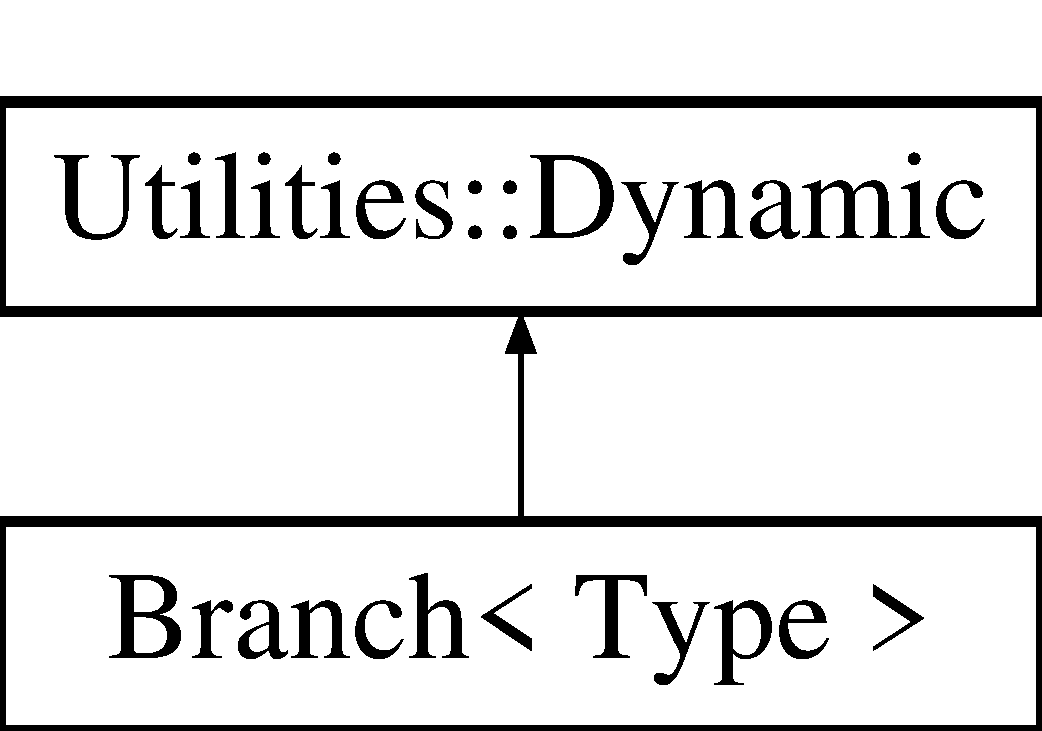
\includegraphics[height=2.000000cm]{classBranch}
\end{center}
\end{figure}
\subsection*{Public Member Functions}
\begin{DoxyCompactItemize}
\item 
\hyperlink{classBranch_aeb963f83cf85bbcdef023ddbc020a46a}{Branch} (T\+Tree $\ast$ttree, T\+String new\+\_\+branch\+\_\+name)
\item 
virtual \hyperlink{classBranch_a75022b7e676e5f675b98c1bf7922dd4e}{$\sim$\+Branch} ()
\item 
Type \hyperlink{classBranch_abe830de2e0e7c0df57fdb51436631e1e}{get\+Value} ()
\item 
void \hyperlink{classBranch_abe26b3df8dc53eeb1770d853a39865b1}{set\+Value} (Type new\+\_\+value)
\item 
void \hyperlink{classBranch_a390e9610f26ce93743237dbe3695b4c1}{set\+Reset\+Value} (Type new\+\_\+reset\+\_\+value)
\item 
void \hyperlink{classBranch_aff52fd008db1471e60107522bc62dfb7}{reset\+Value} ()
\end{DoxyCompactItemize}


\subsection{Constructor \& Destructor Documentation}
\index{Branch@{Branch}!Branch@{Branch}}
\index{Branch@{Branch}!Branch@{Branch}}
\subsubsection[{\texorpdfstring{Branch(\+T\+Tree $\ast$ttree, T\+String new\+\_\+branch\+\_\+name)}{Branch(TTree *ttree, TString new_branch_name)}}]{\setlength{\rightskip}{0pt plus 5cm}template$<$typename Type$>$ {\bf Branch}$<$ Type $>$\+::{\bf Branch} (
\begin{DoxyParamCaption}
\item[{T\+Tree $\ast$}]{ttree, }
\item[{T\+String}]{new\+\_\+branch\+\_\+name}
\end{DoxyParamCaption}
)}\hypertarget{classBranch_aeb963f83cf85bbcdef023ddbc020a46a}{}\label{classBranch_aeb963f83cf85bbcdef023ddbc020a46a}
\hyperlink{classBranch}{Branch} object constructor 
\begin{DoxyTemplParams}{Template Parameters}
{\em Type} & type of branch value \\
\hline
\end{DoxyTemplParams}

\begin{DoxyParams}{Parameters}
{\em ttree} & pointer to T\+Tree \\
\hline
{\em new\+\_\+branch\+\_\+name} & new branch name \\
\hline
\end{DoxyParams}
\begin{DoxyReturn}{Returns}
none 
\end{DoxyReturn}
\index{Branch@{Branch}!````~Branch@{$\sim$\+Branch}}
\index{````~Branch@{$\sim$\+Branch}!Branch@{Branch}}
\subsubsection[{\texorpdfstring{$\sim$\+Branch()}{~Branch()}}]{\setlength{\rightskip}{0pt plus 5cm}template$<$typename Type$>$ virtual {\bf Branch}$<$ Type $>$\+::$\sim${\bf Branch} (
\begin{DoxyParamCaption}
{}
\end{DoxyParamCaption}
)\hspace{0.3cm}{\ttfamily [virtual]}}\hypertarget{classBranch_a75022b7e676e5f675b98c1bf7922dd4e}{}\label{classBranch_a75022b7e676e5f675b98c1bf7922dd4e}
\hyperlink{classBranch}{Branch} object destructor 
\begin{DoxyTemplParams}{Template Parameters}
{\em Type} & type of branch value \\
\hline
\end{DoxyTemplParams}
\begin{DoxyReturn}{Returns}
none 
\end{DoxyReturn}


\subsection{Member Function Documentation}
\index{Branch@{Branch}!get\+Value@{get\+Value}}
\index{get\+Value@{get\+Value}!Branch@{Branch}}
\subsubsection[{\texorpdfstring{get\+Value()}{getValue()}}]{\setlength{\rightskip}{0pt plus 5cm}template$<$typename Type$>$ Type {\bf Branch}$<$ Type $>$\+::get\+Value (
\begin{DoxyParamCaption}
{}
\end{DoxyParamCaption}
)}\hypertarget{classBranch_abe830de2e0e7c0df57fdb51436631e1e}{}\label{classBranch_abe830de2e0e7c0df57fdb51436631e1e}
Get current leaf value 
\begin{DoxyTemplParams}{Template Parameters}
{\em Type} & type of branch value \\
\hline
\end{DoxyTemplParams}
\begin{DoxyReturn}{Returns}
value of current leaf 
\end{DoxyReturn}
\index{Branch@{Branch}!reset\+Value@{reset\+Value}}
\index{reset\+Value@{reset\+Value}!Branch@{Branch}}
\subsubsection[{\texorpdfstring{reset\+Value()}{resetValue()}}]{\setlength{\rightskip}{0pt plus 5cm}template$<$typename Type$>$ void {\bf Branch}$<$ Type $>$\+::reset\+Value (
\begin{DoxyParamCaption}
{}
\end{DoxyParamCaption}
)}\hypertarget{classBranch_aff52fd008db1471e60107522bc62dfb7}{}\label{classBranch_aff52fd008db1471e60107522bc62dfb7}
Reset the current leaf to the reset value 
\begin{DoxyTemplParams}{Template Parameters}
{\em Type} & type of branch value \\
\hline
\end{DoxyTemplParams}
\begin{DoxyReturn}{Returns}
none 
\end{DoxyReturn}
\index{Branch@{Branch}!set\+Reset\+Value@{set\+Reset\+Value}}
\index{set\+Reset\+Value@{set\+Reset\+Value}!Branch@{Branch}}
\subsubsection[{\texorpdfstring{set\+Reset\+Value(\+Type new\+\_\+reset\+\_\+value)}{setResetValue(Type new_reset_value)}}]{\setlength{\rightskip}{0pt plus 5cm}template$<$typename Type$>$ void {\bf Branch}$<$ Type $>$\+::set\+Reset\+Value (
\begin{DoxyParamCaption}
\item[{Type}]{new\+\_\+reset\+\_\+value}
\end{DoxyParamCaption}
)}\hypertarget{classBranch_a390e9610f26ce93743237dbe3695b4c1}{}\label{classBranch_a390e9610f26ce93743237dbe3695b4c1}
Set the reset value of branch 
\begin{DoxyTemplParams}{Template Parameters}
{\em Type} & type of branch value \\
\hline
\end{DoxyTemplParams}

\begin{DoxyParams}{Parameters}
{\em new\+\_\+reset\+\_\+value} & new reset value (e.\+g. -\/999; default is the default type constructor) \\
\hline
\end{DoxyParams}
\begin{DoxyReturn}{Returns}
none 
\end{DoxyReturn}
\index{Branch@{Branch}!set\+Value@{set\+Value}}
\index{set\+Value@{set\+Value}!Branch@{Branch}}
\subsubsection[{\texorpdfstring{set\+Value(\+Type new\+\_\+value)}{setValue(Type new_value)}}]{\setlength{\rightskip}{0pt plus 5cm}template$<$typename Type$>$ void {\bf Branch}$<$ Type $>$\+::set\+Value (
\begin{DoxyParamCaption}
\item[{Type}]{new\+\_\+value}
\end{DoxyParamCaption}
)}\hypertarget{classBranch_abe26b3df8dc53eeb1770d853a39865b1}{}\label{classBranch_abe26b3df8dc53eeb1770d853a39865b1}
Set value of current leaf 
\begin{DoxyTemplParams}{Template Parameters}
{\em Type} & type of branch value \\
\hline
\end{DoxyTemplParams}

\begin{DoxyParams}{Parameters}
{\em new\+\_\+value} & new value \\
\hline
\end{DoxyParams}
\begin{DoxyReturn}{Returns}
none 
\end{DoxyReturn}


The documentation for this class was generated from the following file\+:\begin{DoxyCompactItemize}
\item 
arbol.\+h\end{DoxyCompactItemize}

\hypertarget{classCut}{}\doxysection{Cut Class Reference}
\label{classCut}\index{Cut@{Cut}}


{\ttfamily \#include $<$cutflow.\+h$>$}

\doxysubsection*{Public Member Functions}
\begin{DoxyCompactItemize}
\item 
\mbox{\hyperlink{classCut_aaa89435c5326080296041bc38937ab2d}{Cut}} (std\+::string new\+\_\+name, std\+::function$<$ bool()$>$ new\+\_\+evaluate)
\item 
\mbox{\hyperlink{classCut_adcfec6d2df97f8e84058078f2f736b03}{Cut}} (std\+::string new\+\_\+name, std\+::function$<$ bool()$>$ new\+\_\+evaluate, std\+::function$<$ float()$>$ new\+\_\+compute\+\_\+weight)
\item 
\mbox{\hyperlink{classCut}{Cut}} $\ast$ \mbox{\hyperlink{classCut_a51d128a9d77f6e9e2965ae0a2ea077e1}{clone}} (std\+::string new\+\_\+name)
\item 
void \mbox{\hyperlink{classCut_a9b1298219ed1f85bba920e4049d712e3}{print}} ()
\item 
float \mbox{\hyperlink{classCut_a3201e86949718110994a9301987f0f98}{get\+Weight}} ()
\end{DoxyCompactItemize}
\doxysubsection*{Public Attributes}
\begin{DoxyCompactItemize}
\item 
std\+::string \mbox{\hyperlink{classCut_accf700d2d00746b97a265d4aea3f55c2}{name}}
\item 
std\+::function$<$ bool()$>$ \mbox{\hyperlink{classCut_a4205ad5e62b859536797141f3ace2253}{evaluate}}
\item 
std\+::function$<$ float()$>$ \mbox{\hyperlink{classCut_a908dfdeed9d882ca026427c0942fb999}{compute\+\_\+weight}}
\item 
\mbox{\hyperlink{classCut}{Cut}} $\ast$ \mbox{\hyperlink{classCut_acb046f96bc50db055cccdb1f9a601780}{parent}}
\item 
\mbox{\hyperlink{classCut}{Cut}} $\ast$ \mbox{\hyperlink{classCut_a2142ffe68028bb0c211408c0f5bb8bfb}{right}}
\item 
\mbox{\hyperlink{classCut}{Cut}} $\ast$ \mbox{\hyperlink{classCut_a2c65e372172dfa0f705d117d3ad0f668}{left}}
\item 
int \mbox{\hyperlink{classCut_a01ab47c909e962b3820e2e866c0230a8}{n\+\_\+pass}}
\item 
int \mbox{\hyperlink{classCut_aff7fd0749654bdae7ede4bfbea700c2d}{n\+\_\+fail}}
\item 
float \mbox{\hyperlink{classCut_ac5f58e08d36bad07f9c62ab9c04eb1b7}{n\+\_\+pass\+\_\+weighted}}
\item 
float \mbox{\hyperlink{classCut_ad780ce231646c09c612b14180b2772e0}{n\+\_\+fail\+\_\+weighted}}
\end{DoxyCompactItemize}


\doxysubsection{Detailed Description}
Object that represents a single cut in an analysis 

\doxysubsection{Constructor \& Destructor Documentation}
\mbox{\Hypertarget{classCut_aaa89435c5326080296041bc38937ab2d}\label{classCut_aaa89435c5326080296041bc38937ab2d}} 
\index{Cut@{Cut}!Cut@{Cut}}
\index{Cut@{Cut}!Cut@{Cut}}
\doxysubsubsection{\texorpdfstring{Cut()}{Cut()}\hspace{0.1cm}{\footnotesize\ttfamily [1/2]}}
{\footnotesize\ttfamily Cut\+::\+Cut (\begin{DoxyParamCaption}\item[{std\+::string}]{new\+\_\+name,  }\item[{std\+::function$<$ bool()$>$}]{new\+\_\+evaluate }\end{DoxyParamCaption})}

\mbox{\hyperlink{classCut}{Cut}} object constructor (assumes weight == 1.\+0) 
\begin{DoxyParams}{Parameters}
{\em new\+\_\+name} & new cut name \\
\hline
{\em new\+\_\+evaluate} & lambda function that evaluates new cut conditional logic \\
\hline
\end{DoxyParams}
\begin{DoxyReturn}{Returns}
none 
\end{DoxyReturn}
\mbox{\Hypertarget{classCut_adcfec6d2df97f8e84058078f2f736b03}\label{classCut_adcfec6d2df97f8e84058078f2f736b03}} 
\index{Cut@{Cut}!Cut@{Cut}}
\index{Cut@{Cut}!Cut@{Cut}}
\doxysubsubsection{\texorpdfstring{Cut()}{Cut()}\hspace{0.1cm}{\footnotesize\ttfamily [2/2]}}
{\footnotesize\ttfamily Cut\+::\+Cut (\begin{DoxyParamCaption}\item[{std\+::string}]{new\+\_\+name,  }\item[{std\+::function$<$ bool()$>$}]{new\+\_\+evaluate,  }\item[{std\+::function$<$ float()$>$}]{new\+\_\+compute\+\_\+weight }\end{DoxyParamCaption})}

\mbox{\hyperlink{classCut}{Cut}} object constructor 
\begin{DoxyParams}{Parameters}
{\em new\+\_\+name} & new cut name \\
\hline
{\em new\+\_\+evaluate} & lambda function that evaluates new cut conditional logic \\
\hline
{\em new\+\_\+compute\+\_\+weight} & lambda function that computes event weight \\
\hline
\end{DoxyParams}
\begin{DoxyReturn}{Returns}
none 
\end{DoxyReturn}


\doxysubsection{Member Function Documentation}
\mbox{\Hypertarget{classCut_a51d128a9d77f6e9e2965ae0a2ea077e1}\label{classCut_a51d128a9d77f6e9e2965ae0a2ea077e1}} 
\index{Cut@{Cut}!clone@{clone}}
\index{clone@{clone}!Cut@{Cut}}
\doxysubsubsection{\texorpdfstring{clone()}{clone()}}
{\footnotesize\ttfamily \mbox{\hyperlink{classCut}{Cut}} $\ast$ Cut\+::clone (\begin{DoxyParamCaption}\item[{std\+::string}]{new\+\_\+name }\end{DoxyParamCaption})}

Create a copy of this cut object 
\begin{DoxyParams}{Parameters}
{\em new\+\_\+name} & name of cut copy \\
\hline
\end{DoxyParams}
\begin{DoxyReturn}{Returns}
pointer to a copy of this cut object 
\end{DoxyReturn}
\mbox{\Hypertarget{classCut_a3201e86949718110994a9301987f0f98}\label{classCut_a3201e86949718110994a9301987f0f98}} 
\index{Cut@{Cut}!getWeight@{getWeight}}
\index{getWeight@{getWeight}!Cut@{Cut}}
\doxysubsubsection{\texorpdfstring{getWeight()}{getWeight()}}
{\footnotesize\ttfamily float Cut\+::get\+Weight (\begin{DoxyParamCaption}{ }\end{DoxyParamCaption})}

Get even weight for this cut (on top of previous cut weights) \begin{DoxyReturn}{Returns}
event weight 
\end{DoxyReturn}
\mbox{\Hypertarget{classCut_a9b1298219ed1f85bba920e4049d712e3}\label{classCut_a9b1298219ed1f85bba920e4049d712e3}} 
\index{Cut@{Cut}!print@{print}}
\index{print@{print}!Cut@{Cut}}
\doxysubsubsection{\texorpdfstring{print()}{print()}}
{\footnotesize\ttfamily void Cut\+::print (\begin{DoxyParamCaption}{ }\end{DoxyParamCaption})}

Print cut object properties \begin{DoxyReturn}{Returns}
none 
\end{DoxyReturn}


\doxysubsection{Member Data Documentation}
\mbox{\Hypertarget{classCut_a908dfdeed9d882ca026427c0942fb999}\label{classCut_a908dfdeed9d882ca026427c0942fb999}} 
\index{Cut@{Cut}!compute\_weight@{compute\_weight}}
\index{compute\_weight@{compute\_weight}!Cut@{Cut}}
\doxysubsubsection{\texorpdfstring{compute\_weight}{compute\_weight}}
{\footnotesize\ttfamily std\+::function$<$float()$>$ Cut\+::compute\+\_\+weight}

Lambda function that computes event weight \mbox{\Hypertarget{classCut_a4205ad5e62b859536797141f3ace2253}\label{classCut_a4205ad5e62b859536797141f3ace2253}} 
\index{Cut@{Cut}!evaluate@{evaluate}}
\index{evaluate@{evaluate}!Cut@{Cut}}
\doxysubsubsection{\texorpdfstring{evaluate}{evaluate}}
{\footnotesize\ttfamily std\+::function$<$bool()$>$ Cut\+::evaluate}

Lambda function that evaluates conditional logic (i.\+e. the cut itself) \mbox{\Hypertarget{classCut_a2c65e372172dfa0f705d117d3ad0f668}\label{classCut_a2c65e372172dfa0f705d117d3ad0f668}} 
\index{Cut@{Cut}!left@{left}}
\index{left@{left}!Cut@{Cut}}
\doxysubsubsection{\texorpdfstring{left}{left}}
{\footnotesize\ttfamily \mbox{\hyperlink{classCut}{Cut}}$\ast$ Cut\+::left}

Pointer to next cut to evaluate if this cut evaluates to false \mbox{\Hypertarget{classCut_aff7fd0749654bdae7ede4bfbea700c2d}\label{classCut_aff7fd0749654bdae7ede4bfbea700c2d}} 
\index{Cut@{Cut}!n\_fail@{n\_fail}}
\index{n\_fail@{n\_fail}!Cut@{Cut}}
\doxysubsubsection{\texorpdfstring{n\_fail}{n\_fail}}
{\footnotesize\ttfamily int Cut\+::n\+\_\+fail}

Number of events that fail cut \mbox{\Hypertarget{classCut_ad780ce231646c09c612b14180b2772e0}\label{classCut_ad780ce231646c09c612b14180b2772e0}} 
\index{Cut@{Cut}!n\_fail\_weighted@{n\_fail\_weighted}}
\index{n\_fail\_weighted@{n\_fail\_weighted}!Cut@{Cut}}
\doxysubsubsection{\texorpdfstring{n\_fail\_weighted}{n\_fail\_weighted}}
{\footnotesize\ttfamily float Cut\+::n\+\_\+fail\+\_\+weighted}

Weighted number of events that fail cut \mbox{\Hypertarget{classCut_a01ab47c909e962b3820e2e866c0230a8}\label{classCut_a01ab47c909e962b3820e2e866c0230a8}} 
\index{Cut@{Cut}!n\_pass@{n\_pass}}
\index{n\_pass@{n\_pass}!Cut@{Cut}}
\doxysubsubsection{\texorpdfstring{n\_pass}{n\_pass}}
{\footnotesize\ttfamily int Cut\+::n\+\_\+pass}

Number of events that pass cut \mbox{\Hypertarget{classCut_ac5f58e08d36bad07f9c62ab9c04eb1b7}\label{classCut_ac5f58e08d36bad07f9c62ab9c04eb1b7}} 
\index{Cut@{Cut}!n\_pass\_weighted@{n\_pass\_weighted}}
\index{n\_pass\_weighted@{n\_pass\_weighted}!Cut@{Cut}}
\doxysubsubsection{\texorpdfstring{n\_pass\_weighted}{n\_pass\_weighted}}
{\footnotesize\ttfamily float Cut\+::n\+\_\+pass\+\_\+weighted}

Weighted number of events that pass cut \mbox{\Hypertarget{classCut_accf700d2d00746b97a265d4aea3f55c2}\label{classCut_accf700d2d00746b97a265d4aea3f55c2}} 
\index{Cut@{Cut}!name@{name}}
\index{name@{name}!Cut@{Cut}}
\doxysubsubsection{\texorpdfstring{name}{name}}
{\footnotesize\ttfamily std\+::string Cut\+::name}

Unique name of cut \mbox{\Hypertarget{classCut_acb046f96bc50db055cccdb1f9a601780}\label{classCut_acb046f96bc50db055cccdb1f9a601780}} 
\index{Cut@{Cut}!parent@{parent}}
\index{parent@{parent}!Cut@{Cut}}
\doxysubsubsection{\texorpdfstring{parent}{parent}}
{\footnotesize\ttfamily \mbox{\hyperlink{classCut}{Cut}}$\ast$ Cut\+::parent}

Pointer to parent cut \mbox{\Hypertarget{classCut_a2142ffe68028bb0c211408c0f5bb8bfb}\label{classCut_a2142ffe68028bb0c211408c0f5bb8bfb}} 
\index{Cut@{Cut}!right@{right}}
\index{right@{right}!Cut@{Cut}}
\doxysubsubsection{\texorpdfstring{right}{right}}
{\footnotesize\ttfamily \mbox{\hyperlink{classCut}{Cut}}$\ast$ Cut\+::right}

Pointer to next cut to evaluate if this cut evaluates to true 

The documentation for this class was generated from the following files\+:\begin{DoxyCompactItemize}
\item 
/github/workspace/rapido/src/cutflow.\+h\item 
/github/workspace/rapido/src/cutflow.\+cc\end{DoxyCompactItemize}

\hypertarget{classCutflow}{}\doxysection{Cutflow Class Reference}
\label{classCutflow}\index{Cutflow@{Cutflow}}


{\ttfamily \#include $<$cutflow.\+h$>$}

Inheritance diagram for Cutflow\+:\begin{figure}[H]
\begin{center}
\leavevmode
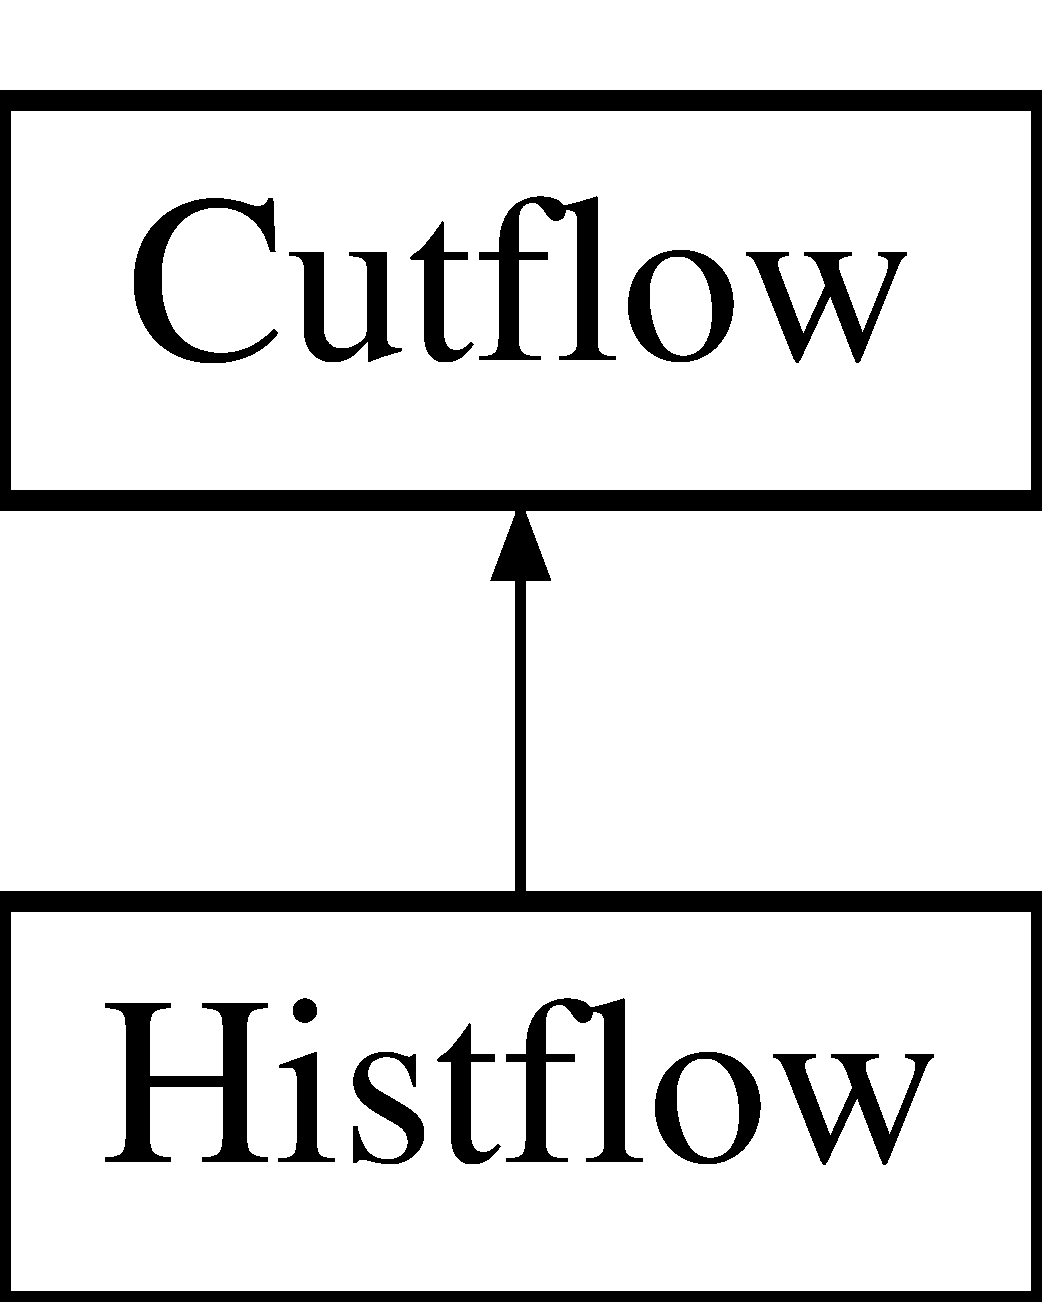
\includegraphics[height=2.000000cm]{classCutflow}
\end{center}
\end{figure}
\doxysubsection*{Public Member Functions}
\begin{DoxyCompactItemize}
\item 
\mbox{\hyperlink{classCutflow_a17811cb40a7906fc65e79ce69e3b21be}{Cutflow}} ()
\item 
\mbox{\hyperlink{classCutflow_a46b6444272c54fe9988e8d328d0644ca}{Cutflow}} (std\+::string new\+\_\+name)
\item 
\mbox{\hyperlink{classCutflow_ae13ef13d8c6cef09bed242855e45aacf}{Cutflow}} (std\+::string new\+\_\+name, \mbox{\hyperlink{classCut}{Cut}} $\ast$new\+\_\+root)
\item 
\mbox{\hyperlink{classCutflow_adb300cd78d57a287934e4d22856a0ffe}{$\sim$\+Cutflow}} ()
\item 
void \mbox{\hyperlink{classCutflow_ad27d37141c3748779a5d81fad919ecbb}{set\+Root}} (\mbox{\hyperlink{classCut}{Cut}} $\ast$new\+\_\+root)
\item 
void \mbox{\hyperlink{classCutflow_a8da46f1053a6b97991489ee0920c29a1}{insert}} (std\+::string target\+\_\+cut\+\_\+name, \mbox{\hyperlink{classCut}{Cut}} $\ast$new\+\_\+cut, Direction direction)
\item 
virtual bool \mbox{\hyperlink{classCutflow_a8fc98b9c006b80db96576c8bdcf6a0a8}{run}} ()
\item 
bool \mbox{\hyperlink{classCutflow_a3b5a6dc6e9490037d190eca691295859}{run\+Until}} (std\+::string target\+\_\+cut\+\_\+name)
\item 
\mbox{\hyperlink{classCut}{Cut}} $\ast$ \mbox{\hyperlink{classCutflow_a11c1116dc01d4c0679945eeff66ff0a4}{find\+Terminus}} (std\+::string starting\+\_\+cut\+\_\+name)
\item 
void \mbox{\hyperlink{classCutflow_a0cb4c8bd6d15ace1f85fe0cfb8d9d828}{print}} ()
\item 
void \mbox{\hyperlink{classCutflow_a43e58326fbce5306e2b3d080c6cd85f0}{write\+CSV}} (std\+::string output\+\_\+dir=\char`\"{}\char`\"{})
\end{DoxyCompactItemize}
\doxysubsection*{Public Attributes}
\begin{DoxyCompactItemize}
\item 
std\+::string \mbox{\hyperlink{classCutflow_a268e204c942ca35895a94f1be7ce111d}{name}}
\item 
\mbox{\hyperlink{classUtilities_1_1Variables}{Utilities\+::\+Variables}} \mbox{\hyperlink{classCutflow_a71390324488ac6ed4a72c41f4a2c1c10}{globals}}
\end{DoxyCompactItemize}
\doxysubsection*{Protected Member Functions}
\begin{DoxyCompactItemize}
\item 
\mbox{\hyperlink{classCut}{Cut}} $\ast$ \mbox{\hyperlink{classCutflow_a20193ee89ee39b0fc58ab4f27e2779db}{get\+Cut}} (std\+::string cut\+\_\+name)
\item 
\mbox{\hyperlink{classCut}{Cut}} $\ast$ \mbox{\hyperlink{classCutflow_a6949f1d9e7d74c6ab8cf0c6f28ac3701}{recursive\+Find\+Terminus}} (\mbox{\hyperlink{classCut}{Cut}} $\ast$cut)
\item 
void \mbox{\hyperlink{classCutflow_a54e6ae7d3e4c9efdb8fd830ab8a0e0e9}{recursive\+Print}} (std\+::string tabs, \mbox{\hyperlink{classCut}{Cut}} $\ast$cut, Direction direction, float weight)
\item 
std\+::pair$<$ \mbox{\hyperlink{classCut}{Cut}} $\ast$, bool $>$ \mbox{\hyperlink{classCutflow_a8298a5ed45d1963271dbe9c7d1f1586f}{recursive\+Evaluate}} (\mbox{\hyperlink{classCut}{Cut}} $\ast$cut)
\item 
void \mbox{\hyperlink{classCutflow_adc7029b27ff8d742d10c75d6f6342dac}{recursive\+Delete}} (\mbox{\hyperlink{classCut}{Cut}} $\ast$cut)
\end{DoxyCompactItemize}
\doxysubsection*{Protected Attributes}
\begin{DoxyCompactItemize}
\item 
\mbox{\hyperlink{classCut}{Cut}} $\ast$ \mbox{\hyperlink{classCutflow_a96f2343bfae77c94f2e87b5f3a128d6d}{root}}
\item 
std\+::map$<$ std\+::string, \mbox{\hyperlink{classCut}{Cut}} $\ast$ $>$ \mbox{\hyperlink{classCutflow_a76f5cbd82750844d379384c7b1243cca}{cut\+\_\+record}}
\end{DoxyCompactItemize}


\doxysubsection{Detailed Description}
An analysis represented as a binary search tree (i.\+e. analysis = tree, cut = node) 

\doxysubsection{Constructor \& Destructor Documentation}
\mbox{\Hypertarget{classCutflow_a17811cb40a7906fc65e79ce69e3b21be}\label{classCutflow_a17811cb40a7906fc65e79ce69e3b21be}} 
\index{Cutflow@{Cutflow}!Cutflow@{Cutflow}}
\index{Cutflow@{Cutflow}!Cutflow@{Cutflow}}
\doxysubsubsection{\texorpdfstring{Cutflow()}{Cutflow()}\hspace{0.1cm}{\footnotesize\ttfamily [1/3]}}
{\footnotesize\ttfamily Cutflow\+::\+Cutflow (\begin{DoxyParamCaption}{ }\end{DoxyParamCaption})}

\mbox{\hyperlink{classCutflow}{Cutflow}} object default constructor \begin{DoxyReturn}{Returns}
none 
\end{DoxyReturn}
\mbox{\Hypertarget{classCutflow_a46b6444272c54fe9988e8d328d0644ca}\label{classCutflow_a46b6444272c54fe9988e8d328d0644ca}} 
\index{Cutflow@{Cutflow}!Cutflow@{Cutflow}}
\index{Cutflow@{Cutflow}!Cutflow@{Cutflow}}
\doxysubsubsection{\texorpdfstring{Cutflow()}{Cutflow()}\hspace{0.1cm}{\footnotesize\ttfamily [2/3]}}
{\footnotesize\ttfamily Cutflow\+::\+Cutflow (\begin{DoxyParamCaption}\item[{std\+::string}]{new\+\_\+name }\end{DoxyParamCaption})}

\mbox{\hyperlink{classCutflow}{Cutflow}} object overload constructor 
\begin{DoxyParams}{Parameters}
{\em new\+\_\+name} & name of cutflow \\
\hline
\end{DoxyParams}
\begin{DoxyReturn}{Returns}
none 
\end{DoxyReturn}
\mbox{\Hypertarget{classCutflow_ae13ef13d8c6cef09bed242855e45aacf}\label{classCutflow_ae13ef13d8c6cef09bed242855e45aacf}} 
\index{Cutflow@{Cutflow}!Cutflow@{Cutflow}}
\index{Cutflow@{Cutflow}!Cutflow@{Cutflow}}
\doxysubsubsection{\texorpdfstring{Cutflow()}{Cutflow()}\hspace{0.1cm}{\footnotesize\ttfamily [3/3]}}
{\footnotesize\ttfamily Cutflow\+::\+Cutflow (\begin{DoxyParamCaption}\item[{std\+::string}]{new\+\_\+name,  }\item[{\mbox{\hyperlink{classCut}{Cut}} $\ast$}]{new\+\_\+root }\end{DoxyParamCaption})}

\mbox{\hyperlink{classCutflow}{Cutflow}} object overload constructor 
\begin{DoxyParams}{Parameters}
{\em new\+\_\+name} & name of cutflow \\
\hline
{\em new\+\_\+root} & pointer to cut object to use as root node \\
\hline
\end{DoxyParams}
\begin{DoxyReturn}{Returns}
none 
\end{DoxyReturn}
\mbox{\Hypertarget{classCutflow_adb300cd78d57a287934e4d22856a0ffe}\label{classCutflow_adb300cd78d57a287934e4d22856a0ffe}} 
\index{Cutflow@{Cutflow}!````~Cutflow@{$\sim$Cutflow}}
\index{````~Cutflow@{$\sim$Cutflow}!Cutflow@{Cutflow}}
\doxysubsubsection{\texorpdfstring{$\sim$Cutflow()}{~Cutflow()}}
{\footnotesize\ttfamily Cutflow\+::$\sim$\+Cutflow (\begin{DoxyParamCaption}{ }\end{DoxyParamCaption})}

\mbox{\hyperlink{classCutflow}{Cutflow}} object destructor \begin{DoxyReturn}{Returns}
none 
\end{DoxyReturn}


\doxysubsection{Member Function Documentation}
\mbox{\Hypertarget{classCutflow_a11c1116dc01d4c0679945eeff66ff0a4}\label{classCutflow_a11c1116dc01d4c0679945eeff66ff0a4}} 
\index{Cutflow@{Cutflow}!findTerminus@{findTerminus}}
\index{findTerminus@{findTerminus}!Cutflow@{Cutflow}}
\doxysubsubsection{\texorpdfstring{findTerminus()}{findTerminus()}}
{\footnotesize\ttfamily \mbox{\hyperlink{classCut}{Cut}} $\ast$ Cutflow\+::find\+Terminus (\begin{DoxyParamCaption}\item[{std\+::string}]{starting\+\_\+cut\+\_\+name }\end{DoxyParamCaption})}

Find the rightmost terminal leaf from a given node 
\begin{DoxyParams}{Parameters}
{\em starting\+\_\+cut\+\_\+name} & cut from which to start search \\
\hline
\end{DoxyParams}
\begin{DoxyReturn}{Returns}
terminal cut 
\end{DoxyReturn}
\mbox{\Hypertarget{classCutflow_a20193ee89ee39b0fc58ab4f27e2779db}\label{classCutflow_a20193ee89ee39b0fc58ab4f27e2779db}} 
\index{Cutflow@{Cutflow}!getCut@{getCut}}
\index{getCut@{getCut}!Cutflow@{Cutflow}}
\doxysubsubsection{\texorpdfstring{getCut()}{getCut()}}
{\footnotesize\ttfamily \mbox{\hyperlink{classCut}{Cut}} $\ast$ Cutflow\+::get\+Cut (\begin{DoxyParamCaption}\item[{std\+::string}]{cut\+\_\+name }\end{DoxyParamCaption})\hspace{0.3cm}{\ttfamily [protected]}}

(PROTECTED) Retrieve cut object from cut record 
\begin{DoxyParams}{Parameters}
{\em cut\+\_\+name} & cut name \\
\hline
\end{DoxyParams}
\begin{DoxyReturn}{Returns}
pointer to cut 
\end{DoxyReturn}
\mbox{\Hypertarget{classCutflow_a8da46f1053a6b97991489ee0920c29a1}\label{classCutflow_a8da46f1053a6b97991489ee0920c29a1}} 
\index{Cutflow@{Cutflow}!insert@{insert}}
\index{insert@{insert}!Cutflow@{Cutflow}}
\doxysubsubsection{\texorpdfstring{insert()}{insert()}}
{\footnotesize\ttfamily void Cutflow\+::insert (\begin{DoxyParamCaption}\item[{std\+::string}]{target\+\_\+cut\+\_\+name,  }\item[{\mbox{\hyperlink{classCut}{Cut}} $\ast$}]{new\+\_\+cut,  }\item[{Direction}]{direction }\end{DoxyParamCaption})}

Insert a new node AFTER a given node 
\begin{DoxyParams}{Parameters}
{\em target\+\_\+cut\+\_\+name} & target node name \\
\hline
{\em new\+\_\+cut} & pointer to new node \\
\hline
{\em direction} & direction (Left/false, Right/true) \\
\hline
\end{DoxyParams}
\begin{DoxyReturn}{Returns}
none 
\end{DoxyReturn}
\mbox{\Hypertarget{classCutflow_a0cb4c8bd6d15ace1f85fe0cfb8d9d828}\label{classCutflow_a0cb4c8bd6d15ace1f85fe0cfb8d9d828}} 
\index{Cutflow@{Cutflow}!print@{print}}
\index{print@{print}!Cutflow@{Cutflow}}
\doxysubsubsection{\texorpdfstring{print()}{print()}}
{\footnotesize\ttfamily void Cutflow\+::print (\begin{DoxyParamCaption}{ }\end{DoxyParamCaption})}

Print cutflow \begin{DoxyReturn}{Returns}
none 
\end{DoxyReturn}
\mbox{\Hypertarget{classCutflow_adc7029b27ff8d742d10c75d6f6342dac}\label{classCutflow_adc7029b27ff8d742d10c75d6f6342dac}} 
\index{Cutflow@{Cutflow}!recursiveDelete@{recursiveDelete}}
\index{recursiveDelete@{recursiveDelete}!Cutflow@{Cutflow}}
\doxysubsubsection{\texorpdfstring{recursiveDelete()}{recursiveDelete()}}
{\footnotesize\ttfamily void Cutflow\+::recursive\+Delete (\begin{DoxyParamCaption}\item[{\mbox{\hyperlink{classCut}{Cut}} $\ast$}]{cut }\end{DoxyParamCaption})\hspace{0.3cm}{\ttfamily [protected]}}

(PROTECTED) Recursively delete cuts in the cutflow 
\begin{DoxyParams}{Parameters}
{\em cut} & pointer to current cut \\
\hline
\end{DoxyParams}
\begin{DoxyReturn}{Returns}
none 
\end{DoxyReturn}
\mbox{\Hypertarget{classCutflow_a8298a5ed45d1963271dbe9c7d1f1586f}\label{classCutflow_a8298a5ed45d1963271dbe9c7d1f1586f}} 
\index{Cutflow@{Cutflow}!recursiveEvaluate@{recursiveEvaluate}}
\index{recursiveEvaluate@{recursiveEvaluate}!Cutflow@{Cutflow}}
\doxysubsubsection{\texorpdfstring{recursiveEvaluate()}{recursiveEvaluate()}}
{\footnotesize\ttfamily std\+::pair$<$ \mbox{\hyperlink{classCut}{Cut}} $\ast$, bool $>$ Cutflow\+::recursive\+Evaluate (\begin{DoxyParamCaption}\item[{\mbox{\hyperlink{classCut}{Cut}} $\ast$}]{cut }\end{DoxyParamCaption})\hspace{0.3cm}{\ttfamily [protected]}}

(PROTECTED) Recursively evaulate cuts in the cutflow 
\begin{DoxyParams}{Parameters}
{\em cut} & pointer to current cut \\
\hline
\end{DoxyParams}
\begin{DoxyReturn}{Returns}
std\+::pair of a pointer to terminal cut and a boolean (true = pass, false = fail) 
\end{DoxyReturn}
\mbox{\Hypertarget{classCutflow_a6949f1d9e7d74c6ab8cf0c6f28ac3701}\label{classCutflow_a6949f1d9e7d74c6ab8cf0c6f28ac3701}} 
\index{Cutflow@{Cutflow}!recursiveFindTerminus@{recursiveFindTerminus}}
\index{recursiveFindTerminus@{recursiveFindTerminus}!Cutflow@{Cutflow}}
\doxysubsubsection{\texorpdfstring{recursiveFindTerminus()}{recursiveFindTerminus()}}
{\footnotesize\ttfamily \mbox{\hyperlink{classCut}{Cut}} $\ast$ Cutflow\+::recursive\+Find\+Terminus (\begin{DoxyParamCaption}\item[{\mbox{\hyperlink{classCut}{Cut}} $\ast$}]{cut }\end{DoxyParamCaption})\hspace{0.3cm}{\ttfamily [protected]}}

(PROTECTED) Recursively search for the rightmost terminal leaf from a given node 
\begin{DoxyParams}{Parameters}
{\em cut} & pointer to current cut \\
\hline
\end{DoxyParams}
\begin{DoxyReturn}{Returns}
terminal cut 
\end{DoxyReturn}
\mbox{\Hypertarget{classCutflow_a54e6ae7d3e4c9efdb8fd830ab8a0e0e9}\label{classCutflow_a54e6ae7d3e4c9efdb8fd830ab8a0e0e9}} 
\index{Cutflow@{Cutflow}!recursivePrint@{recursivePrint}}
\index{recursivePrint@{recursivePrint}!Cutflow@{Cutflow}}
\doxysubsubsection{\texorpdfstring{recursivePrint()}{recursivePrint()}}
{\footnotesize\ttfamily void Cutflow\+::recursive\+Print (\begin{DoxyParamCaption}\item[{std\+::string}]{tabs,  }\item[{\mbox{\hyperlink{classCut}{Cut}} $\ast$}]{cut,  }\item[{Direction}]{direction,  }\item[{float}]{weight }\end{DoxyParamCaption})\hspace{0.3cm}{\ttfamily [protected]}}

(PROTECTED) Recursively print cuts 
\begin{DoxyParams}{Parameters}
{\em tabs} & string with the prefix tabs for current cut \\
\hline
{\em cut} & pointer to current cut \\
\hline
{\em direction} & direction of cut relative to parent \\
\hline
{\em weight} & current event weight \\
\hline
\end{DoxyParams}
\begin{DoxyReturn}{Returns}
none 
\end{DoxyReturn}
\mbox{\Hypertarget{classCutflow_a8fc98b9c006b80db96576c8bdcf6a0a8}\label{classCutflow_a8fc98b9c006b80db96576c8bdcf6a0a8}} 
\index{Cutflow@{Cutflow}!run@{run}}
\index{run@{run}!Cutflow@{Cutflow}}
\doxysubsubsection{\texorpdfstring{run()}{run()}}
{\footnotesize\ttfamily bool Cutflow\+::run (\begin{DoxyParamCaption}{ }\end{DoxyParamCaption})\hspace{0.3cm}{\ttfamily [virtual]}}

Run cutflow until any terminus \begin{DoxyReturn}{Returns}
whether or not the terminal cut in the cutflow passed 
\end{DoxyReturn}


Reimplemented in \mbox{\hyperlink{classHistflow_a675b897276d33e146d1c2707023f1edd}{Histflow}}.

\mbox{\Hypertarget{classCutflow_a3b5a6dc6e9490037d190eca691295859}\label{classCutflow_a3b5a6dc6e9490037d190eca691295859}} 
\index{Cutflow@{Cutflow}!runUntil@{runUntil}}
\index{runUntil@{runUntil}!Cutflow@{Cutflow}}
\doxysubsubsection{\texorpdfstring{runUntil()}{runUntil()}}
{\footnotesize\ttfamily bool Cutflow\+::run\+Until (\begin{DoxyParamCaption}\item[{std\+::string}]{target\+\_\+cut\+\_\+name }\end{DoxyParamCaption})}

Run cutflow until a target terminal cut \begin{DoxySeeAlso}{See also}
\mbox{\hyperlink{classCutflow_a3b5a6dc6e9490037d190eca691295859}{Cutflow\+::run\+Until}} 
\end{DoxySeeAlso}

\begin{DoxyParams}{Parameters}
{\em target\+\_\+cut\+\_\+name} & name of target cut \\
\hline
\end{DoxyParams}
\begin{DoxyReturn}{Returns}
whether or not (true/false) the target cut was reached and passed 
\end{DoxyReturn}
\mbox{\Hypertarget{classCutflow_ad27d37141c3748779a5d81fad919ecbb}\label{classCutflow_ad27d37141c3748779a5d81fad919ecbb}} 
\index{Cutflow@{Cutflow}!setRoot@{setRoot}}
\index{setRoot@{setRoot}!Cutflow@{Cutflow}}
\doxysubsubsection{\texorpdfstring{setRoot()}{setRoot()}}
{\footnotesize\ttfamily void Cutflow\+::set\+Root (\begin{DoxyParamCaption}\item[{\mbox{\hyperlink{classCut}{Cut}} $\ast$}]{new\+\_\+root }\end{DoxyParamCaption})}

Set root node of cutflow object 
\begin{DoxyParams}{Parameters}
{\em new\+\_\+root} & pointer to cut object to use as new root node \\
\hline
\end{DoxyParams}
\begin{DoxyReturn}{Returns}
none 
\end{DoxyReturn}
\mbox{\Hypertarget{classCutflow_a43e58326fbce5306e2b3d080c6cd85f0}\label{classCutflow_a43e58326fbce5306e2b3d080c6cd85f0}} 
\index{Cutflow@{Cutflow}!writeCSV@{writeCSV}}
\index{writeCSV@{writeCSV}!Cutflow@{Cutflow}}
\doxysubsubsection{\texorpdfstring{writeCSV()}{writeCSV()}}
{\footnotesize\ttfamily void Cutflow\+::write\+CSV (\begin{DoxyParamCaption}\item[{std\+::string}]{output\+\_\+dir = {\ttfamily \char`\"{}\char`\"{}} }\end{DoxyParamCaption})}

Print all cutflow paths to separate CSV files \{output\+\_\+dir\}/\{name\}\+\_\+\{terminal\+\_\+cut\}.csv 
\begin{DoxyParams}{Parameters}
{\em output\+\_\+dir} & target directory for output CSV files (optional) \\
\hline
\end{DoxyParams}
\begin{DoxyReturn}{Returns}
none 
\end{DoxyReturn}


\doxysubsection{Member Data Documentation}
\mbox{\Hypertarget{classCutflow_a76f5cbd82750844d379384c7b1243cca}\label{classCutflow_a76f5cbd82750844d379384c7b1243cca}} 
\index{Cutflow@{Cutflow}!cut\_record@{cut\_record}}
\index{cut\_record@{cut\_record}!Cutflow@{Cutflow}}
\doxysubsubsection{\texorpdfstring{cut\_record}{cut\_record}}
{\footnotesize\ttfamily std\+::map$<$std\+::string, \mbox{\hyperlink{classCut}{Cut}}$\ast$$>$ Cutflow\+::cut\+\_\+record\hspace{0.3cm}{\ttfamily [protected]}}

Map (\char`\"{}record\char`\"{}) of all cuts in cutflow \mbox{\Hypertarget{classCutflow_a71390324488ac6ed4a72c41f4a2c1c10}\label{classCutflow_a71390324488ac6ed4a72c41f4a2c1c10}} 
\index{Cutflow@{Cutflow}!globals@{globals}}
\index{globals@{globals}!Cutflow@{Cutflow}}
\doxysubsubsection{\texorpdfstring{globals}{globals}}
{\footnotesize\ttfamily \mbox{\hyperlink{classUtilities_1_1Variables}{Utilities\+::\+Variables}} Cutflow\+::globals}

Dynamic list of variables to track across object scope (i.\+e. psuedo-\/members) \mbox{\Hypertarget{classCutflow_a268e204c942ca35895a94f1be7ce111d}\label{classCutflow_a268e204c942ca35895a94f1be7ce111d}} 
\index{Cutflow@{Cutflow}!name@{name}}
\index{name@{name}!Cutflow@{Cutflow}}
\doxysubsubsection{\texorpdfstring{name}{name}}
{\footnotesize\ttfamily std\+::string Cutflow\+::name}

Name of cutflow \mbox{\Hypertarget{classCutflow_a96f2343bfae77c94f2e87b5f3a128d6d}\label{classCutflow_a96f2343bfae77c94f2e87b5f3a128d6d}} 
\index{Cutflow@{Cutflow}!root@{root}}
\index{root@{root}!Cutflow@{Cutflow}}
\doxysubsubsection{\texorpdfstring{root}{root}}
{\footnotesize\ttfamily \mbox{\hyperlink{classCut}{Cut}}$\ast$ Cutflow\+::root\hspace{0.3cm}{\ttfamily [protected]}}

Pointer to cut that is used as the root node 

The documentation for this class was generated from the following files\+:\begin{DoxyCompactItemize}
\item 
/\+Users/jguiang/\+Projects/rapido/src/cutflow.\+h\item 
/\+Users/jguiang/\+Projects/rapido/src/cutflow.\+cc\end{DoxyCompactItemize}

\hypertarget{classUtilities_1_1Dynamic}{}\doxysection{Utilities\+::Dynamic Class Reference}
\label{classUtilities_1_1Dynamic}\index{Utilities::Dynamic@{Utilities::Dynamic}}


{\ttfamily \#include $<$utilities.\+h$>$}

Inheritance diagram for Utilities\+::Dynamic\+:\begin{figure}[H]
\begin{center}
\leavevmode
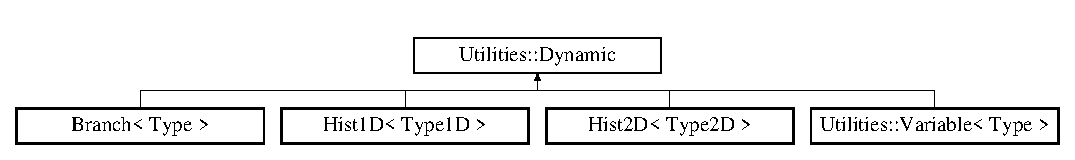
\includegraphics[height=1.696970cm]{classUtilities_1_1Dynamic}
\end{center}
\end{figure}
\doxysubsection*{Public Member Functions}
\begin{DoxyCompactItemize}
\item 
virtual \mbox{\hyperlink{classUtilities_1_1Dynamic_a4d12e083a7d3fceec2d390f47df3b992}{$\sim$\+Dynamic}} ()
\end{DoxyCompactItemize}


\doxysubsection{Detailed Description}
\char`\"{}\+Dynamic\char`\"{} object that serves as a base for templated objects 

\doxysubsection{Constructor \& Destructor Documentation}
\mbox{\Hypertarget{classUtilities_1_1Dynamic_a4d12e083a7d3fceec2d390f47df3b992}\label{classUtilities_1_1Dynamic_a4d12e083a7d3fceec2d390f47df3b992}} 
\index{Utilities::Dynamic@{Utilities::Dynamic}!````~Dynamic@{$\sim$Dynamic}}
\index{````~Dynamic@{$\sim$Dynamic}!Utilities::Dynamic@{Utilities::Dynamic}}
\doxysubsubsection{\texorpdfstring{$\sim$Dynamic()}{~Dynamic()}}
{\footnotesize\ttfamily virtual Utilities\+::\+Dynamic\+::$\sim$\+Dynamic (\begin{DoxyParamCaption}{ }\end{DoxyParamCaption})\hspace{0.3cm}{\ttfamily [virtual]}}

\mbox{\hyperlink{classUtilities_1_1Dynamic}{Dynamic}} object destructor \begin{DoxyReturn}{Returns}
none 
\end{DoxyReturn}


The documentation for this class was generated from the following file\+:\begin{DoxyCompactItemize}
\item 
/\+Users/jguiang/\+Projects/rapido/utilities.\+h\end{DoxyCompactItemize}

\hypertarget{classLooper}{}\doxysection{Looper Class Reference}
\label{classLooper}\index{Looper@{Looper}}


{\ttfamily \#include $<$looper.\+h$>$}

\doxysubsection*{Public Member Functions}
\begin{DoxyCompactItemize}
\item 
\mbox{\hyperlink{classLooper_a916868e8a7a8bf73274a82bf47df22f4}{Looper}} (TChain $\ast$new\+\_\+tchain)
\item 
virtual \mbox{\hyperlink{classLooper_a23ff9511f1d99ca1f3753e59a1b3a22b}{$\sim$\+Looper}} ()
\item 
void \mbox{\hyperlink{classLooper_a8b259a7ad0c2aa45ae49d1ec08d37af0}{run}} (std\+::function$<$ void(TTree $\ast$ttree)$>$ init, std\+::function$<$ void(int entry)$>$ eval)
\end{DoxyCompactItemize}
\doxysubsection*{Public Attributes}
\begin{DoxyCompactItemize}
\item 
TChain $\ast$ \mbox{\hyperlink{classLooper_ae804a8c01aea03c415a0277099b7a2a0}{tchain}}
\item 
TString \mbox{\hyperlink{classLooper_aa42e5d8d2e16cf7768ea5d582a17868c}{ttree\+\_\+name}}
\item 
unsigned int \mbox{\hyperlink{classLooper_ab368e58278fc91c4814e579cb9080d4f}{current\+\_\+entry}}
\item 
unsigned int \mbox{\hyperlink{classLooper_abbf626538aced372130172ac86958265}{n\+\_\+events\+\_\+processed}}
\item 
unsigned int \mbox{\hyperlink{classLooper_a6251eeff0d36df11886ac1a50521a1db}{n\+\_\+events\+\_\+to\+\_\+process}}
\end{DoxyCompactItemize}


\doxysubsection{Detailed Description}
Object to handle looping over ROOT files 

\doxysubsection{Constructor \& Destructor Documentation}
\mbox{\Hypertarget{classLooper_a916868e8a7a8bf73274a82bf47df22f4}\label{classLooper_a916868e8a7a8bf73274a82bf47df22f4}} 
\index{Looper@{Looper}!Looper@{Looper}}
\index{Looper@{Looper}!Looper@{Looper}}
\doxysubsubsection{\texorpdfstring{Looper()}{Looper()}}
{\footnotesize\ttfamily Looper\+::\+Looper (\begin{DoxyParamCaption}\item[{TChain $\ast$}]{new\+\_\+tchain }\end{DoxyParamCaption})}

\mbox{\hyperlink{classLooper}{Looper}} object constructor 
\begin{DoxyParams}{Parameters}
{\em new\+\_\+tchain} & pointer to ROOT TChain of files to loop over \\
\hline
\end{DoxyParams}
\begin{DoxyReturn}{Returns}
none 
\end{DoxyReturn}
\mbox{\Hypertarget{classLooper_a23ff9511f1d99ca1f3753e59a1b3a22b}\label{classLooper_a23ff9511f1d99ca1f3753e59a1b3a22b}} 
\index{Looper@{Looper}!````~Looper@{$\sim$Looper}}
\index{````~Looper@{$\sim$Looper}!Looper@{Looper}}
\doxysubsubsection{\texorpdfstring{$\sim$Looper()}{~Looper()}}
{\footnotesize\ttfamily virtual Looper\+::$\sim$\+Looper (\begin{DoxyParamCaption}{ }\end{DoxyParamCaption})\hspace{0.3cm}{\ttfamily [virtual]}}

\mbox{\hyperlink{classLooper}{Looper}} object destructor \begin{DoxyReturn}{Returns}
none 
\end{DoxyReturn}


\doxysubsection{Member Function Documentation}
\mbox{\Hypertarget{classLooper_a8b259a7ad0c2aa45ae49d1ec08d37af0}\label{classLooper_a8b259a7ad0c2aa45ae49d1ec08d37af0}} 
\index{Looper@{Looper}!run@{run}}
\index{run@{run}!Looper@{Looper}}
\doxysubsubsection{\texorpdfstring{run()}{run()}}
{\footnotesize\ttfamily void Looper\+::run (\begin{DoxyParamCaption}\item[{std\+::function$<$ void(TTree $\ast$ttree)$>$}]{init,  }\item[{std\+::function$<$ void(int entry)$>$}]{eval }\end{DoxyParamCaption})}

Run looper with file-\/ and event-\/processing logic captured in void lambda functions.

The following example uses a class named \char`\"{}\+Selector\char`\"{} generated by ROOT\+::\+Make\+Selector; this class requires certain file-\/ and event-\/processing initialization steps\+: 
\begin{DoxyCode}{0}
\DoxyCodeLine{\textcolor{keywordtype}{int} main()}
\DoxyCodeLine{\{}
\DoxyCodeLine{    TChain* \mbox{\hyperlink{classLooper_ae804a8c01aea03c415a0277099b7a2a0}{tchain}} = \textcolor{keyword}{new} TChain(\textcolor{stringliteral}{"{}Events"{}});}
\DoxyCodeLine{    \mbox{\hyperlink{classLooper_ae804a8c01aea03c415a0277099b7a2a0}{tchain}}-\/>Add(\textcolor{stringliteral}{"{}/path/to/file.root"{}});}
\DoxyCodeLine{    selector = Selector(); \textcolor{comment}{// generated by ROOT::MakeSelector}}
\DoxyCodeLine{    looper = \mbox{\hyperlink{classLooper_a916868e8a7a8bf73274a82bf47df22f4}{Looper}}(\mbox{\hyperlink{classLooper_ae804a8c01aea03c415a0277099b7a2a0}{tchain}}, \textcolor{stringliteral}{"{}Events"{}});}
\DoxyCodeLine{    looper.run(}
\DoxyCodeLine{        [\&](TTree* ttree) \{ selector.Init(ttree); \},}
\DoxyCodeLine{        [\&](\textcolor{keywordtype}{int} entry) }
\DoxyCodeLine{        \{}
\DoxyCodeLine{            selector.GetEntry(entry);}
\DoxyCodeLine{            selector.Process(entry);}
\DoxyCodeLine{            \textcolor{comment}{// -\/> insert your favorite cutflow here <-\/-\/}}
\DoxyCodeLine{        \}}
\DoxyCodeLine{    );}
\DoxyCodeLine{\}}

\end{DoxyCode}
 
\begin{DoxyParams}{Parameters}
{\em init} & file-\/level initialization steps captured in a void lambda function \\
\hline
{\em eval} & event-\/level logic captured in a void lambda function \\
\hline
\end{DoxyParams}
\begin{DoxyReturn}{Returns}
none 
\end{DoxyReturn}


\doxysubsection{Member Data Documentation}
\mbox{\Hypertarget{classLooper_ab368e58278fc91c4814e579cb9080d4f}\label{classLooper_ab368e58278fc91c4814e579cb9080d4f}} 
\index{Looper@{Looper}!current\_entry@{current\_entry}}
\index{current\_entry@{current\_entry}!Looper@{Looper}}
\doxysubsubsection{\texorpdfstring{current\_entry}{current\_entry}}
{\footnotesize\ttfamily unsigned int Looper\+::current\+\_\+entry}

Current entry in TTree (i.\+e. current index of event loop) \mbox{\Hypertarget{classLooper_abbf626538aced372130172ac86958265}\label{classLooper_abbf626538aced372130172ac86958265}} 
\index{Looper@{Looper}!n\_events\_processed@{n\_events\_processed}}
\index{n\_events\_processed@{n\_events\_processed}!Looper@{Looper}}
\doxysubsubsection{\texorpdfstring{n\_events\_processed}{n\_events\_processed}}
{\footnotesize\ttfamily unsigned int Looper\+::n\+\_\+events\+\_\+processed}

Number of events that have been processed \mbox{\Hypertarget{classLooper_a6251eeff0d36df11886ac1a50521a1db}\label{classLooper_a6251eeff0d36df11886ac1a50521a1db}} 
\index{Looper@{Looper}!n\_events\_to\_process@{n\_events\_to\_process}}
\index{n\_events\_to\_process@{n\_events\_to\_process}!Looper@{Looper}}
\doxysubsubsection{\texorpdfstring{n\_events\_to\_process}{n\_events\_to\_process}}
{\footnotesize\ttfamily unsigned int Looper\+::n\+\_\+events\+\_\+to\+\_\+process}

Number of events in the TChain \mbox{\Hypertarget{classLooper_ae804a8c01aea03c415a0277099b7a2a0}\label{classLooper_ae804a8c01aea03c415a0277099b7a2a0}} 
\index{Looper@{Looper}!tchain@{tchain}}
\index{tchain@{tchain}!Looper@{Looper}}
\doxysubsubsection{\texorpdfstring{tchain}{tchain}}
{\footnotesize\ttfamily TChain$\ast$ Looper\+::tchain}

ROOT TChain of files to loop over \mbox{\Hypertarget{classLooper_aa42e5d8d2e16cf7768ea5d582a17868c}\label{classLooper_aa42e5d8d2e16cf7768ea5d582a17868c}} 
\index{Looper@{Looper}!ttree\_name@{ttree\_name}}
\index{ttree\_name@{ttree\_name}!Looper@{Looper}}
\doxysubsubsection{\texorpdfstring{ttree\_name}{ttree\_name}}
{\footnotesize\ttfamily TString Looper\+::ttree\+\_\+name}

ROOT TTree name 

The documentation for this class was generated from the following file\+:\begin{DoxyCompactItemize}
\item 
/github/workspace/rapido/src/looper.\+h\end{DoxyCompactItemize}

\hypertarget{classUtilities_1_1Variable}{}\section{Utilities\+:\+:Variable$<$ Type $>$ Class Template Reference}
\label{classUtilities_1_1Variable}\index{Utilities\+::\+Variable$<$ Type $>$@{Utilities\+::\+Variable$<$ Type $>$}}
Inheritance diagram for Utilities\+:\+:Variable$<$ Type $>$\+:\begin{figure}[H]
\begin{center}
\leavevmode
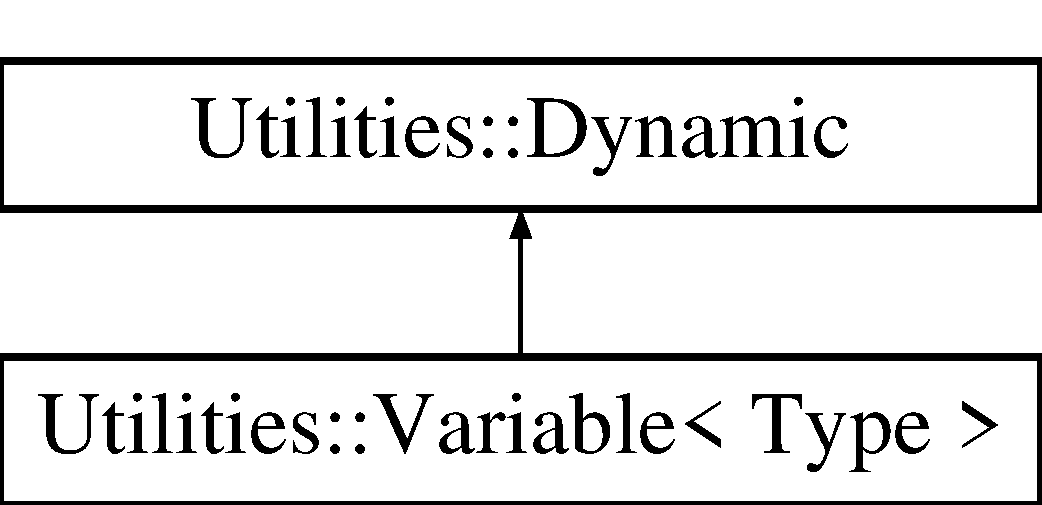
\includegraphics[height=2.000000cm]{classUtilities_1_1Variable}
\end{center}
\end{figure}
\subsection*{Public Member Functions}
\begin{DoxyCompactItemize}
\item 
\hyperlink{classUtilities_1_1Variable_af6f55d5d5c2472b25212828c66b730bc}{Variable} (Type new\+\_\+value)
\item 
virtual \hyperlink{classUtilities_1_1Variable_a4d2bce0bd082e8464b9f193d1e908e0a}{$\sim$\+Variable} ()
\item 
Type \hyperlink{classUtilities_1_1Variable_a2531a59e087062fab302cf487b6bdfa2}{get\+Value} ()
\item 
Type \& \hyperlink{classUtilities_1_1Variable_aec9b6becdc76afca1635280ab81ac41d}{get\+Reference} ()
\item 
void \hyperlink{classUtilities_1_1Variable_af218f1c4f50cbb2f69cc66e8150e05b3}{set\+Value} (Type new\+\_\+value)
\end{DoxyCompactItemize}
\subsection*{Protected Attributes}
\begin{DoxyCompactItemize}
\item 
Type \hyperlink{classUtilities_1_1Variable_ab91417296eea0614f336941a2ecc2944}{value}
\end{DoxyCompactItemize}


\subsection{Constructor \& Destructor Documentation}
\index{Utilities\+::\+Variable@{Utilities\+::\+Variable}!Variable@{Variable}}
\index{Variable@{Variable}!Utilities\+::\+Variable@{Utilities\+::\+Variable}}
\subsubsection[{\texorpdfstring{Variable(\+Type new\+\_\+value)}{Variable(Type new_value)}}]{\setlength{\rightskip}{0pt plus 5cm}template$<$typename Type$>$ {\bf Utilities\+::\+Variable}$<$ Type $>$\+::{\bf Variable} (
\begin{DoxyParamCaption}
\item[{Type}]{new\+\_\+value}
\end{DoxyParamCaption}
)}\hypertarget{classUtilities_1_1Variable_af6f55d5d5c2472b25212828c66b730bc}{}\label{classUtilities_1_1Variable_af6f55d5d5c2472b25212828c66b730bc}
\hyperlink{classUtilities_1_1Variable}{Variable} object constructor 
\begin{DoxyTemplParams}{Template Parameters}
{\em Type} & type of variable \\
\hline
\end{DoxyTemplParams}

\begin{DoxyParams}{Parameters}
{\em new\+\_\+value} & value of new variable \\
\hline
\end{DoxyParams}
\begin{DoxyReturn}{Returns}
none 
\end{DoxyReturn}
\index{Utilities\+::\+Variable@{Utilities\+::\+Variable}!````~Variable@{$\sim$\+Variable}}
\index{````~Variable@{$\sim$\+Variable}!Utilities\+::\+Variable@{Utilities\+::\+Variable}}
\subsubsection[{\texorpdfstring{$\sim$\+Variable()}{~Variable()}}]{\setlength{\rightskip}{0pt plus 5cm}template$<$typename Type$>$ virtual {\bf Utilities\+::\+Variable}$<$ Type $>$\+::$\sim${\bf Variable} (
\begin{DoxyParamCaption}
{}
\end{DoxyParamCaption}
)\hspace{0.3cm}{\ttfamily [virtual]}}\hypertarget{classUtilities_1_1Variable_a4d2bce0bd082e8464b9f193d1e908e0a}{}\label{classUtilities_1_1Variable_a4d2bce0bd082e8464b9f193d1e908e0a}
\hyperlink{classUtilities_1_1Variable}{Variable} object destructor 
\begin{DoxyTemplParams}{Template Parameters}
{\em Type} & type of variable \\
\hline
\end{DoxyTemplParams}
\begin{DoxyReturn}{Returns}
none 
\end{DoxyReturn}


\subsection{Member Function Documentation}
\index{Utilities\+::\+Variable@{Utilities\+::\+Variable}!get\+Reference@{get\+Reference}}
\index{get\+Reference@{get\+Reference}!Utilities\+::\+Variable@{Utilities\+::\+Variable}}
\subsubsection[{\texorpdfstring{get\+Reference()}{getReference()}}]{\setlength{\rightskip}{0pt plus 5cm}template$<$typename Type$>$ Type\& {\bf Utilities\+::\+Variable}$<$ Type $>$\+::get\+Reference (
\begin{DoxyParamCaption}
{}
\end{DoxyParamCaption}
)}\hypertarget{classUtilities_1_1Variable_aec9b6becdc76afca1635280ab81ac41d}{}\label{classUtilities_1_1Variable_aec9b6becdc76afca1635280ab81ac41d}
Get current value by reference 
\begin{DoxyTemplParams}{Template Parameters}
{\em Type} & type of variable \\
\hline
\end{DoxyTemplParams}
\begin{DoxyReturn}{Returns}
value of current leaf 
\end{DoxyReturn}
\index{Utilities\+::\+Variable@{Utilities\+::\+Variable}!get\+Value@{get\+Value}}
\index{get\+Value@{get\+Value}!Utilities\+::\+Variable@{Utilities\+::\+Variable}}
\subsubsection[{\texorpdfstring{get\+Value()}{getValue()}}]{\setlength{\rightskip}{0pt plus 5cm}template$<$typename Type$>$ Type {\bf Utilities\+::\+Variable}$<$ Type $>$\+::get\+Value (
\begin{DoxyParamCaption}
{}
\end{DoxyParamCaption}
)}\hypertarget{classUtilities_1_1Variable_a2531a59e087062fab302cf487b6bdfa2}{}\label{classUtilities_1_1Variable_a2531a59e087062fab302cf487b6bdfa2}
Get current value 
\begin{DoxyTemplParams}{Template Parameters}
{\em Type} & type of variable \\
\hline
\end{DoxyTemplParams}
\begin{DoxyReturn}{Returns}
value of current leaf 
\end{DoxyReturn}
\index{Utilities\+::\+Variable@{Utilities\+::\+Variable}!set\+Value@{set\+Value}}
\index{set\+Value@{set\+Value}!Utilities\+::\+Variable@{Utilities\+::\+Variable}}
\subsubsection[{\texorpdfstring{set\+Value(\+Type new\+\_\+value)}{setValue(Type new_value)}}]{\setlength{\rightskip}{0pt plus 5cm}template$<$typename Type$>$ void {\bf Utilities\+::\+Variable}$<$ Type $>$\+::set\+Value (
\begin{DoxyParamCaption}
\item[{Type}]{new\+\_\+value}
\end{DoxyParamCaption}
)}\hypertarget{classUtilities_1_1Variable_af218f1c4f50cbb2f69cc66e8150e05b3}{}\label{classUtilities_1_1Variable_af218f1c4f50cbb2f69cc66e8150e05b3}
Set value of variable 
\begin{DoxyTemplParams}{Template Parameters}
{\em Type} & type of variable \\
\hline
\end{DoxyTemplParams}

\begin{DoxyParams}{Parameters}
{\em new\+\_\+value} & new value \\
\hline
\end{DoxyParams}
\begin{DoxyReturn}{Returns}
none 
\end{DoxyReturn}


\subsection{Member Data Documentation}
\index{Utilities\+::\+Variable@{Utilities\+::\+Variable}!value@{value}}
\index{value@{value}!Utilities\+::\+Variable@{Utilities\+::\+Variable}}
\subsubsection[{\texorpdfstring{value}{value}}]{\setlength{\rightskip}{0pt plus 5cm}template$<$typename Type$>$ Type {\bf Utilities\+::\+Variable}$<$ Type $>$\+::value\hspace{0.3cm}{\ttfamily [protected]}}\hypertarget{classUtilities_1_1Variable_ab91417296eea0614f336941a2ecc2944}{}\label{classUtilities_1_1Variable_ab91417296eea0614f336941a2ecc2944}
\char`\"{}\+Dynamic\char`\"{} variable 

The documentation for this class was generated from the following file\+:\begin{DoxyCompactItemize}
\item 
utilities.\+h\end{DoxyCompactItemize}

\hypertarget{classUtilities_1_1Variables}{}\doxysection{Utilities\+::Variables Class Reference}
\label{classUtilities_1_1Variables}\index{Utilities::Variables@{Utilities::Variables}}


{\ttfamily \#include $<$utilities.\+h$>$}

\doxysubsection*{Public Member Functions}
\begin{DoxyCompactItemize}
\item 
\mbox{\hyperlink{classUtilities_1_1Variables_a60ebf236218fbefc48cb35e6dcabb2d6}{Variables}} ()
\item 
virtual \mbox{\hyperlink{classUtilities_1_1Variables_a4a67d0d360d70d7a928be6fe48c6753b}{$\sim$\+Variables}} ()
\item 
{\footnotesize template$<$typename Type $>$ }\\void \mbox{\hyperlink{classUtilities_1_1Variables_a7763fc000f45ef3956d61fdf2f783130}{new\+Var}} (std\+::string new\+\_\+name)
\item 
{\footnotesize template$<$typename Type $>$ }\\void \mbox{\hyperlink{classUtilities_1_1Variables_a67029a527f5810a298fc6538b6a634d2}{new\+Var}} (std\+::string new\+\_\+name, Type new\+\_\+value)
\item 
{\footnotesize template$<$typename Type $>$ }\\Type \mbox{\hyperlink{classUtilities_1_1Variables_adff493c2ea6249294a35204fd6b3f852}{get\+Var}} (std\+::string name)
\item 
{\footnotesize template$<$typename Type $>$ }\\Type \& \mbox{\hyperlink{classUtilities_1_1Variables_a58011fc344bd7d5eeb70eaa794f8bb78}{get\+Ref}} (std\+::string name)
\item 
{\footnotesize template$<$typename Type $>$ }\\Type \mbox{\hyperlink{classUtilities_1_1Variables_ad5f59cff15b008435763a81bdac8bcf3}{set\+Var}} (std\+::string name, Type new\+\_\+value)
\end{DoxyCompactItemize}
\doxysubsection*{Protected Member Functions}
\begin{DoxyCompactItemize}
\item 
{\footnotesize template$<$typename Type $>$ }\\\mbox{\hyperlink{classUtilities_1_1Variable}{Variable}}$<$ Type $>$ $\ast$ \mbox{\hyperlink{classUtilities_1_1Variables_a609f89b273fec84499bf782a6109e8f2}{get\+Variable}} (std\+::string name)
\end{DoxyCompactItemize}
\doxysubsection*{Protected Attributes}
\begin{DoxyCompactItemize}
\item 
std\+::map$<$ std\+::string, \mbox{\hyperlink{classUtilities_1_1Dynamic}{Dynamic}} $\ast$ $>$ \mbox{\hyperlink{classUtilities_1_1Variables_acd0a2a9ec3135923b460cdf4e571d478}{variables}}
\end{DoxyCompactItemize}


\doxysubsection{Detailed Description}
A group of \char`\"{}dynamic\char`\"{} variables 

\doxysubsection{Constructor \& Destructor Documentation}
\mbox{\Hypertarget{classUtilities_1_1Variables_a60ebf236218fbefc48cb35e6dcabb2d6}\label{classUtilities_1_1Variables_a60ebf236218fbefc48cb35e6dcabb2d6}} 
\index{Utilities::Variables@{Utilities::Variables}!Variables@{Variables}}
\index{Variables@{Variables}!Utilities::Variables@{Utilities::Variables}}
\doxysubsubsection{\texorpdfstring{Variables()}{Variables()}}
{\footnotesize\ttfamily Utilities\+::\+Variables\+::\+Variables (\begin{DoxyParamCaption}{ }\end{DoxyParamCaption})}

\mbox{\hyperlink{classUtilities_1_1Variables}{Variables}} object constructor \begin{DoxyReturn}{Returns}
none 
\end{DoxyReturn}
\mbox{\Hypertarget{classUtilities_1_1Variables_a4a67d0d360d70d7a928be6fe48c6753b}\label{classUtilities_1_1Variables_a4a67d0d360d70d7a928be6fe48c6753b}} 
\index{Utilities::Variables@{Utilities::Variables}!````~Variables@{$\sim$Variables}}
\index{````~Variables@{$\sim$Variables}!Utilities::Variables@{Utilities::Variables}}
\doxysubsubsection{\texorpdfstring{$\sim$Variables()}{~Variables()}}
{\footnotesize\ttfamily virtual Utilities\+::\+Variables\+::$\sim$\+Variables (\begin{DoxyParamCaption}{ }\end{DoxyParamCaption})\hspace{0.3cm}{\ttfamily [virtual]}}

\mbox{\hyperlink{classUtilities_1_1Variables}{Variables}} object destructor \begin{DoxyReturn}{Returns}
none 
\end{DoxyReturn}


\doxysubsection{Member Function Documentation}
\mbox{\Hypertarget{classUtilities_1_1Variables_a58011fc344bd7d5eeb70eaa794f8bb78}\label{classUtilities_1_1Variables_a58011fc344bd7d5eeb70eaa794f8bb78}} 
\index{Utilities::Variables@{Utilities::Variables}!getRef@{getRef}}
\index{getRef@{getRef}!Utilities::Variables@{Utilities::Variables}}
\doxysubsubsection{\texorpdfstring{getRef()}{getRef()}}
{\footnotesize\ttfamily template$<$typename Type $>$ \\
Type \& Utilities\+::\+Variables\+::get\+Ref (\begin{DoxyParamCaption}\item[{std\+::string}]{name }\end{DoxyParamCaption})}

Get variable in map by reference if it exists 
\begin{DoxyTemplParams}{Template Parameters}
{\em Type} & type of variable \\
\hline
\end{DoxyTemplParams}

\begin{DoxyParams}{Parameters}
{\em name} & name of variable \\
\hline
\end{DoxyParams}
\begin{DoxyReturn}{Returns}
none 
\end{DoxyReturn}
\mbox{\Hypertarget{classUtilities_1_1Variables_adff493c2ea6249294a35204fd6b3f852}\label{classUtilities_1_1Variables_adff493c2ea6249294a35204fd6b3f852}} 
\index{Utilities::Variables@{Utilities::Variables}!getVar@{getVar}}
\index{getVar@{getVar}!Utilities::Variables@{Utilities::Variables}}
\doxysubsubsection{\texorpdfstring{getVar()}{getVar()}}
{\footnotesize\ttfamily template$<$typename Type $>$ \\
Type Utilities\+::\+Variables\+::get\+Var (\begin{DoxyParamCaption}\item[{std\+::string}]{name }\end{DoxyParamCaption})}

Get value of a variable in map if it exists 
\begin{DoxyTemplParams}{Template Parameters}
{\em Type} & type of variable \\
\hline
\end{DoxyTemplParams}

\begin{DoxyParams}{Parameters}
{\em name} & name of variable \\
\hline
\end{DoxyParams}
\begin{DoxyReturn}{Returns}
none 
\end{DoxyReturn}
\mbox{\Hypertarget{classUtilities_1_1Variables_a609f89b273fec84499bf782a6109e8f2}\label{classUtilities_1_1Variables_a609f89b273fec84499bf782a6109e8f2}} 
\index{Utilities::Variables@{Utilities::Variables}!getVariable@{getVariable}}
\index{getVariable@{getVariable}!Utilities::Variables@{Utilities::Variables}}
\doxysubsubsection{\texorpdfstring{getVariable()}{getVariable()}}
{\footnotesize\ttfamily template$<$typename Type $>$ \\
\mbox{\hyperlink{classUtilities_1_1Variable}{Variable}}$<$ Type $>$ $\ast$ Utilities\+::\+Variables\+::get\+Variable (\begin{DoxyParamCaption}\item[{std\+::string}]{name }\end{DoxyParamCaption})\hspace{0.3cm}{\ttfamily [protected]}}

(PROTECTED) Retrieve variable object from map if it exists 
\begin{DoxyTemplParams}{Template Parameters}
{\em Type} & type of variable \\
\hline
\end{DoxyTemplParams}

\begin{DoxyParams}{Parameters}
{\em name} & name of variable \\
\hline
\end{DoxyParams}
\begin{DoxyReturn}{Returns}
none 
\end{DoxyReturn}
\mbox{\Hypertarget{classUtilities_1_1Variables_a7763fc000f45ef3956d61fdf2f783130}\label{classUtilities_1_1Variables_a7763fc000f45ef3956d61fdf2f783130}} 
\index{Utilities::Variables@{Utilities::Variables}!newVar@{newVar}}
\index{newVar@{newVar}!Utilities::Variables@{Utilities::Variables}}
\doxysubsubsection{\texorpdfstring{newVar()}{newVar()}\hspace{0.1cm}{\footnotesize\ttfamily [1/2]}}
{\footnotesize\ttfamily template$<$typename Type $>$ \\
void Utilities\+::\+Variables\+::new\+Var (\begin{DoxyParamCaption}\item[{std\+::string}]{new\+\_\+name }\end{DoxyParamCaption})}

Add blank variable to map 
\begin{DoxyTemplParams}{Template Parameters}
{\em Type} & type of new variable \\
\hline
\end{DoxyTemplParams}

\begin{DoxyParams}{Parameters}
{\em new\+\_\+name} & name of new variable \\
\hline
\end{DoxyParams}
\begin{DoxyReturn}{Returns}
none 
\end{DoxyReturn}
\mbox{\Hypertarget{classUtilities_1_1Variables_a67029a527f5810a298fc6538b6a634d2}\label{classUtilities_1_1Variables_a67029a527f5810a298fc6538b6a634d2}} 
\index{Utilities::Variables@{Utilities::Variables}!newVar@{newVar}}
\index{newVar@{newVar}!Utilities::Variables@{Utilities::Variables}}
\doxysubsubsection{\texorpdfstring{newVar()}{newVar()}\hspace{0.1cm}{\footnotesize\ttfamily [2/2]}}
{\footnotesize\ttfamily template$<$typename Type $>$ \\
void Utilities\+::\+Variables\+::new\+Var (\begin{DoxyParamCaption}\item[{std\+::string}]{new\+\_\+name,  }\item[{Type}]{new\+\_\+value }\end{DoxyParamCaption})}

Add new variable to map 
\begin{DoxyTemplParams}{Template Parameters}
{\em Type} & type of new variable \\
\hline
\end{DoxyTemplParams}

\begin{DoxyParams}{Parameters}
{\em new\+\_\+name} & name of new variable \\
\hline
{\em new\+\_\+value} & value of new variable \\
\hline
\end{DoxyParams}
\begin{DoxyReturn}{Returns}
none 
\end{DoxyReturn}
\mbox{\Hypertarget{classUtilities_1_1Variables_ad5f59cff15b008435763a81bdac8bcf3}\label{classUtilities_1_1Variables_ad5f59cff15b008435763a81bdac8bcf3}} 
\index{Utilities::Variables@{Utilities::Variables}!setVar@{setVar}}
\index{setVar@{setVar}!Utilities::Variables@{Utilities::Variables}}
\doxysubsubsection{\texorpdfstring{setVar()}{setVar()}}
{\footnotesize\ttfamily template$<$typename Type $>$ \\
Type Utilities\+::\+Variables\+::set\+Var (\begin{DoxyParamCaption}\item[{std\+::string}]{name,  }\item[{Type}]{new\+\_\+value }\end{DoxyParamCaption})}

Set value of a variable in map if it exists 
\begin{DoxyTemplParams}{Template Parameters}
{\em Type} & type of variable \\
\hline
\end{DoxyTemplParams}

\begin{DoxyParams}{Parameters}
{\em name} & name of variable \\
\hline
{\em new\+\_\+value} & new value for variable \\
\hline
\end{DoxyParams}
\begin{DoxyReturn}{Returns}
none 
\end{DoxyReturn}


\doxysubsection{Member Data Documentation}
\mbox{\Hypertarget{classUtilities_1_1Variables_acd0a2a9ec3135923b460cdf4e571d478}\label{classUtilities_1_1Variables_acd0a2a9ec3135923b460cdf4e571d478}} 
\index{Utilities::Variables@{Utilities::Variables}!variables@{variables}}
\index{variables@{variables}!Utilities::Variables@{Utilities::Variables}}
\doxysubsubsection{\texorpdfstring{variables}{variables}}
{\footnotesize\ttfamily std\+::map$<$std\+::string, \mbox{\hyperlink{classUtilities_1_1Dynamic}{Dynamic}}$\ast$$>$ Utilities\+::\+Variables\+::variables\hspace{0.3cm}{\ttfamily [protected]}}

Map of dynamic variables 

The documentation for this class was generated from the following file\+:\begin{DoxyCompactItemize}
\item 
/\+Users/jguiang/\+Projects/rapido/utilities.\+h\end{DoxyCompactItemize}

%--- End generated contents ---

% Index
\backmatter
\newpage
\phantomsection
\clearemptydoublepage
\addcontentsline{toc}{chapter}{Index}
\printindex

\end{document}
